% #############################################################################
% This is Chapter 3
% !TEX root = ../main.tex
% #############################################################################
% Change the Name of the Chapter i the following line
\fancychapter{Case Study}
\cleardoublepage
% The following line allows to ref this chapter
\label{chap:architecture}


In the last chapter we presented some of the most important models in the literature regarding the prediction of power consumption in buildings. In this chapter, we present in detail the challenge proposed by \ac{EDP}, and the procedure carried out throughout the development of this thesis.

\section{Problem statement and framework}\label{chap3:sec:problem_statement}

The proposed objective for this work is to create a system capable of computing predictions regarding the available power in a building, 5, 10 and 15 minutes ahead. Since all the experiment is directly related to the behavior of a specific building, it makes sense to present the building and its characteristics. Then, it is important to describe the whole procedure carried out in the development of this thesis, from the data processing stage to the comparison between different models.

\section{The building}\label{chap3:sec:building}

The building provided by \ac{EDP} for the development o this research has a total useful area of 39,801$m^2$ distributed in 5 major categories, office area, parking area, technical area, gymnasium area and bar, with the first two areas representing 89\% of the total area of the building. In Figure \ref{consedp} there is a diagram that shows the distribution of energy consumption by type of final use in each area of the building, for the year of 2016.

\begin{figure}[h!]
    \centering
    \begin{center}
    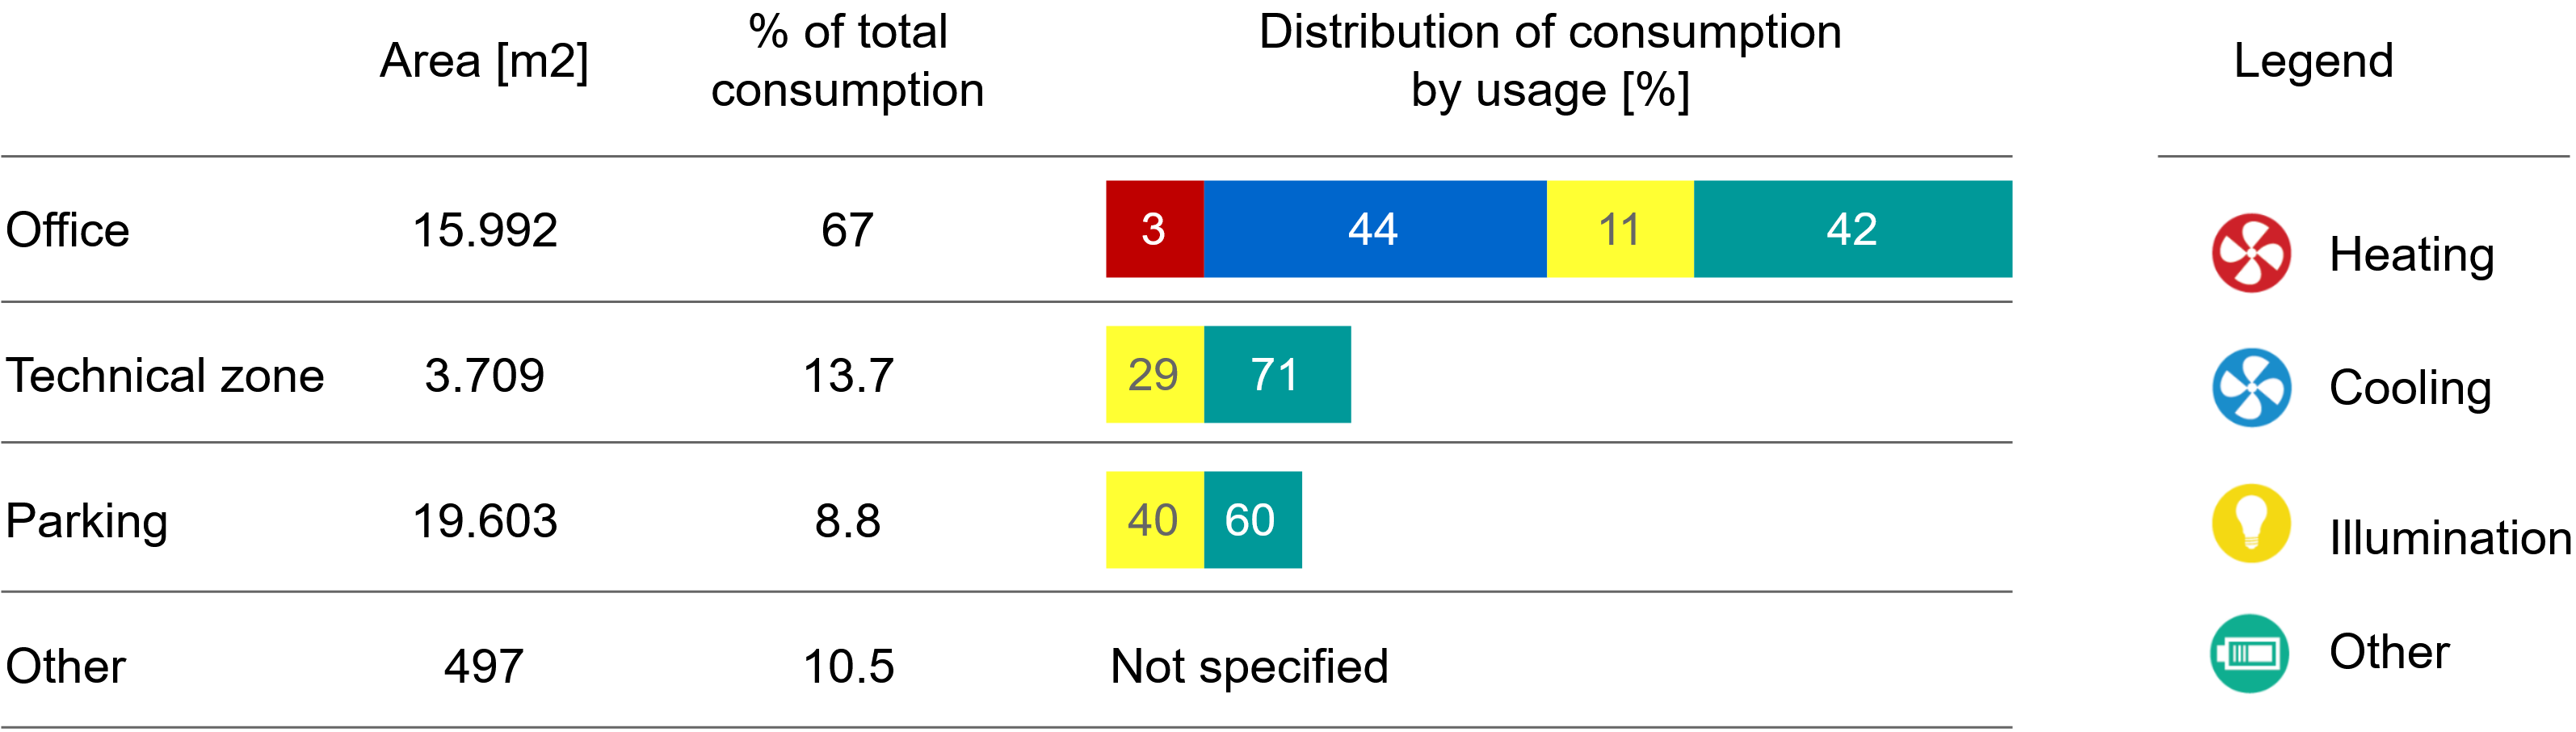
\includegraphics[width=1\textwidth]{Images/ConsumoEDP.png}
    \caption{Energy consumption for the building typology(s) with the highest consumption (2016).}
    \label{consedp}
    \end{center}
\end{figure}
In Figure \ref{consedp} it can be seen that the \ac{HVAC} system represents almost 50\% of the consumption in the office zone. The use of the \ac{HVAC} system is directly related to the external weather conditions. In contrast to the commercial buildings referenced in section \ref{c}, since 44\% of the consumption is connected to the office cooling process, it can be deduced that in the region where this building is located, in warmer years, the consumption of the office area is higher, contributing to an increase in the total consumption of the building. It can also be seen that only 11\% of consumption is due to the lighting of the office area. On the other hand, 42\% of the consumption in the office area is made up of all other factors such as energy plugs. The technical zones represent about 14\% of the total consumption of the building although they represent a small portion of the total area of the building. Most of the consumption performed in these areas is identified as "other" and concerns servers and technical material of the high energy consumption, hence the enormous representativeness of these zones in the total consumption of the building. Parking lots also represent a significant portion of the total consumption of the building. It should be noted that 60\% of consumption is also identified as "other". This portion mainly concerns the electric car charging procedure, that is carried out in the building's garage, managed by the \ac{EVCS}, addressed in Chapter \ref{chap:intro}. This system consists of a total of 13 charging stations for \ac{EV}s, and falls into the category of controllable consumption, i.e., the system can control the power used in vehicle charging, based on the priority level of each vehicle (such as the percentage of full battery charged), and the total power available in the building. The contribution of this thesis falls exactly in this category. Although the system has instantaneous information of the available power state in the building, it would be of great use to have information regarding the future state of available power. In this sense, the work developed in this dissertation aims to respond to this need, contributing to the optimization of the current system.

Modeling energy consumption behaviour and identifying patterns can be crucial both to minimize power usage, and to develop new methodologies to optimize resources. Figure \ref{consumption} illustrates the energy consumption profile of \ac{EDP}'s building in Lisbon, Portugal, during the month of February 2020. The profile illustrated in Figure \ref{consumption} shows a movement that one can identify as a trend. The data presented provides power consumption details for 4 weeks and 4 weekends. The behaviour of the profile tends to be cyclical with a 7 day period. 
\begin{figure}[h!]
    \centering
    \begin{center}
    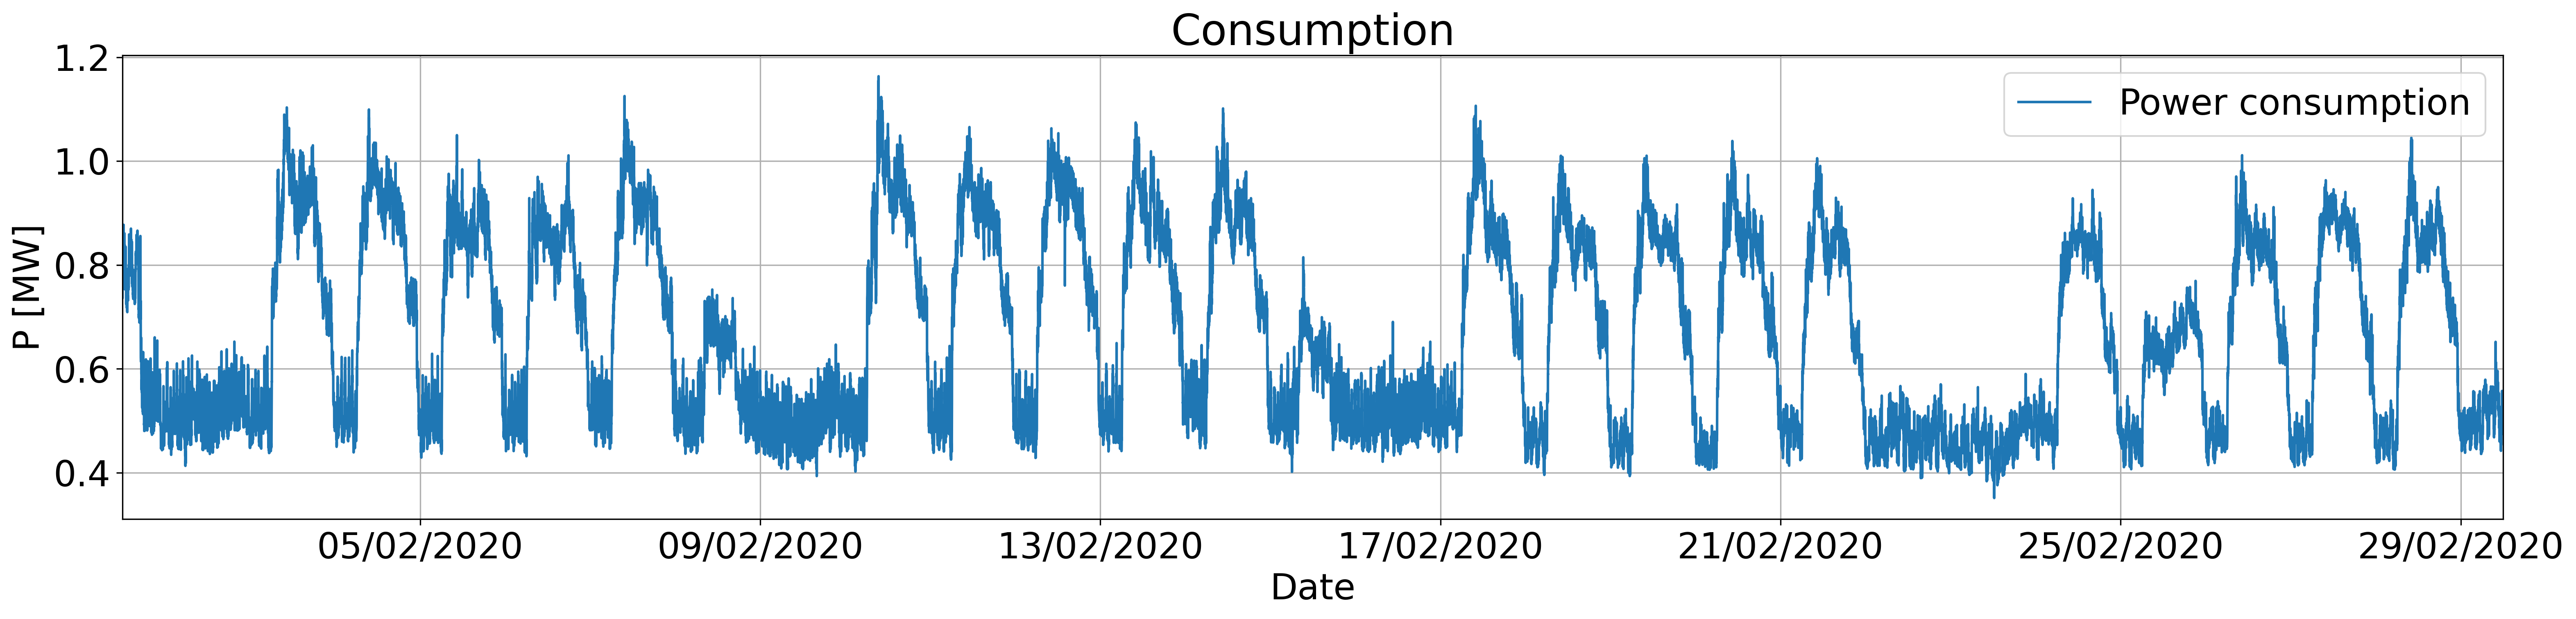
\includegraphics[width=1\textwidth]{Images/power_consumption.png}
    \caption{EDP's building's a) consumption.}
    \label{consumption}
    \end{center}
\end{figure}


Variables that present a trend are more easily examined since it is sometimes possible to associate a cause with their cyclical behavior. By identifying this cause, it becomes not only easier to control its current behavior, but also to predict its future behavior. 

%Power consumption forecasting for buildings is a well know area of research. According to \cite{CivilEU}, Energy consumption forecasting plays a significant role in plans to improve energy performance, save energy and reduce the hazardous environmental impact. Moreover, forecasting also plays a vital role in decision-making and future planning which rely on accurate forecasting results. The ability to predict the available power of any building has many interesting utilities. 

As far as power production is concerned, the building is equipped with a total of 500$m^2$ of \ac{PV} panels area on its roof. The efficiency of the installed panels is around 15$\%$, which represents a total of 70 kWp (kilowatt "peak") of solar generation. Although this kind of production is not controllable, since it depends solely on weather conditions, there are several relationships that can be established by having access to meteorological information. The increase in production generated by the \ac{PV} panels, directly represents an increase in the available power to consume. This factor then becomes an important indicator in the development of this thesis, since its behaviour directly influences the the amount of power available to charge \ac{EV}s. In Figure \ref{production}, one may see the power production profile for the same building and time-interval as Figure \ref{consumption}. The \ac{PV} production behaviour is also cyclical but presents a daily period due to the fact that solar radiation is not influenced by the occupancy rate of the building, so it has no direct relation with the day of the week, but with the hour of the day instead.

\begin{figure}[h!]
    \centering
    \begin{center}
    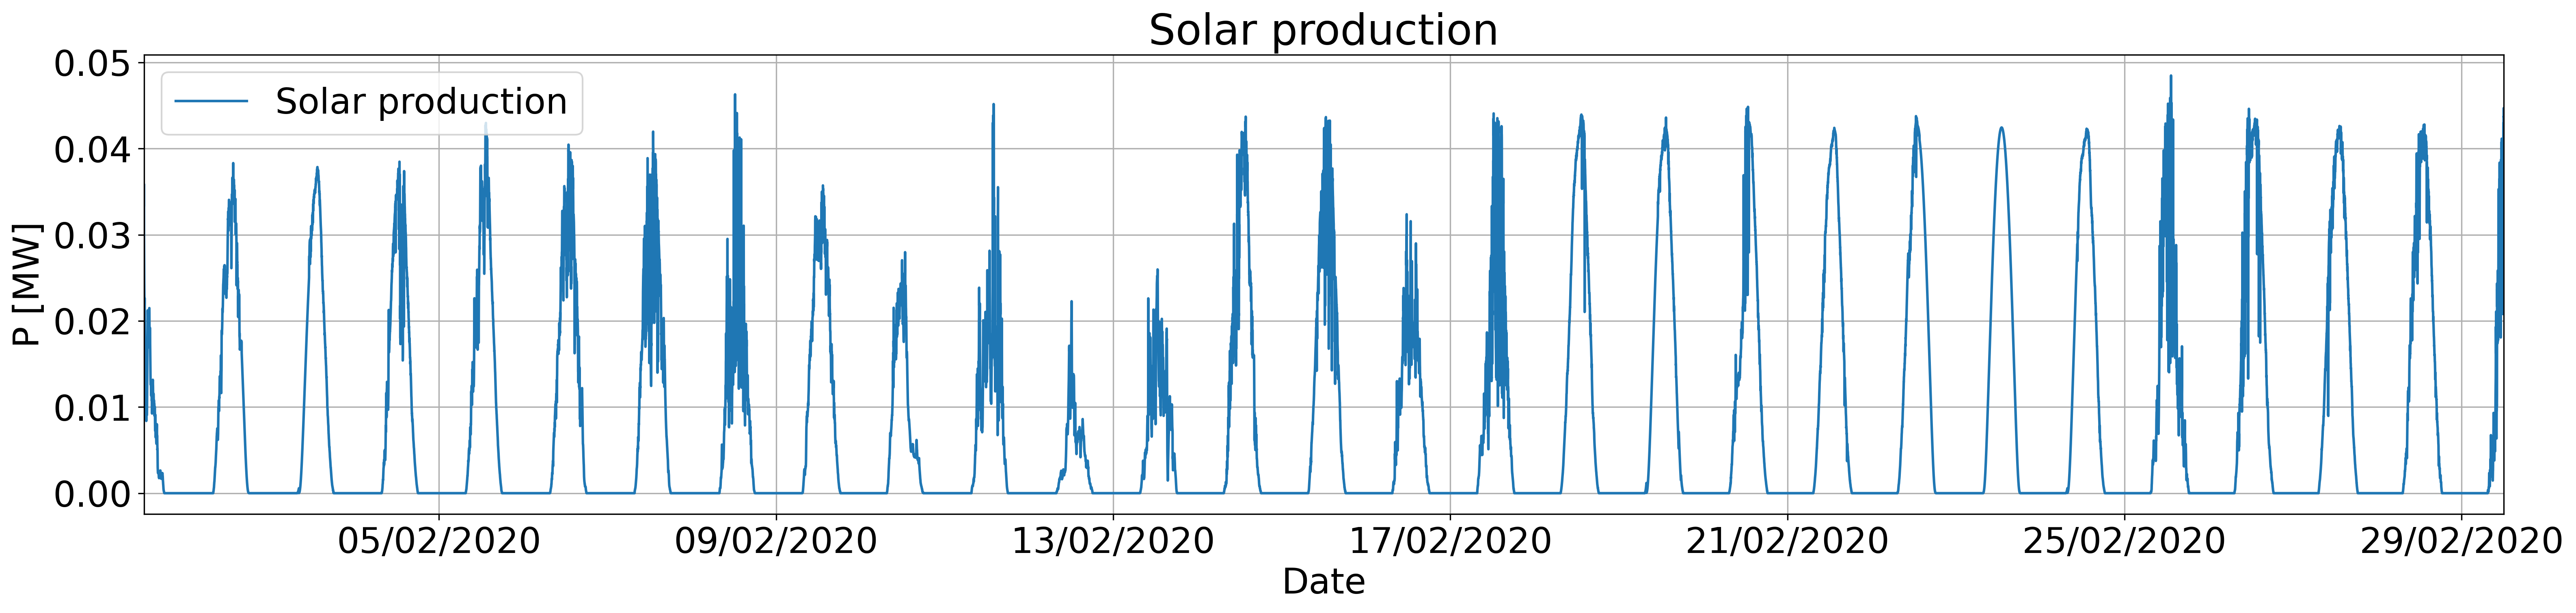
\includegraphics[width=1\textwidth]{Images/power_production.png}
    \caption{EDP's building's a) production.}
    \label{production}
    \end{center}
\end{figure}


Both power consumption and power production are vital information to have in order to predict power available at each time in the building. With this information, there are multiple innovative ideas that can be implemented with the goal of having a more sustainable and power-optimized building.

\section{Proposed variable to predict}\label{chap3:sec:variable_to_predict}

The available power is a key factor because it is the indicator provided to the \ac{EVCS} that enables it to proceed with the optimization of the distribution of the available power by the \ac{EV}s present in the building's garage, which need to be charged.

The power available is not a measured variable, it is a calculated variable. When it comes to computing it, one question then arises: Should one compute the available power and then predict it, or should one predict both consumed power and produced solar power, and just then perform the calculations to find the available power? Figure \ref{avsol} represents two possible solutions for this problem. The first solution consists in creating a model that has as input, besides the other variables, two variables: consumption power and solar production. This model will have as output a forecast for these two variables, and only then is the available power calculated. The second solution is to compute the available power before inputting the data into the model, which causes a reduction in the number of inputs and outputs in the model. 

\begin{figure}[h!]
    \centering
    \begin{center}
    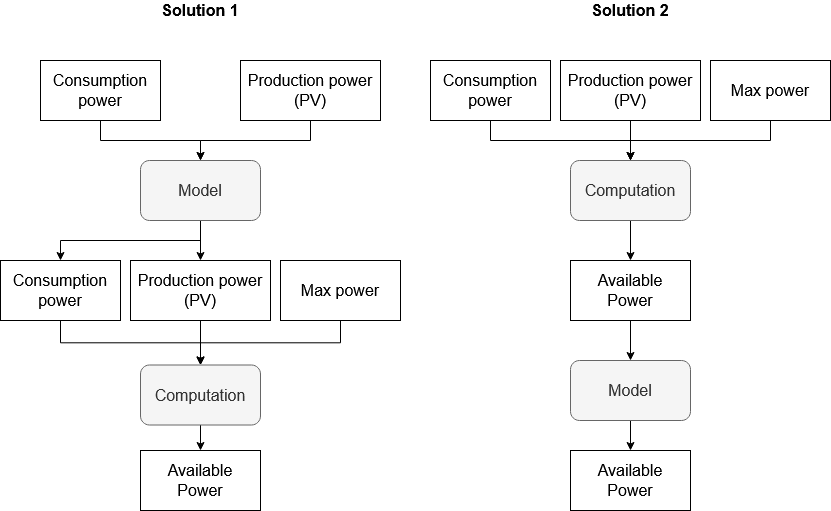
\includegraphics[width=1\textwidth]{Images/Available.png}
    \caption{Model solutions.}
    \label{avsol}
    \end{center}
\end{figure}

Comparing the two proposed hypotheses, solution 1 presents the advantage of predicting two different variables allowing better data manipulation, offering more flexibility. Since the model produces separate results for the consumption and production variables, the amount of possible uses for this data is greater than the amount of possibilities provided by solution 2. On the other hand, solution 2 presents, first of all, the advantage of having a much simpler architecture which makes the user's work easier, and secondly, the main advantage is that it requires the model to predict only one variable and not two. This factor is quite relevant, namely regarding the time it takes the system to produce forecasts, and also the computational capacity that is required from the hardware to allow the prediction of two variables simultaneously. The prediction of two variables with the same model also has the disadvantage of making it difficult to evaluate the behavior of the proposed solution, since a specific model can be very good for predicting one of the variables and bad for the other. 
Taking all these factors into account, the second approach was then chosen, which facilitates the user's work, allows to produce results more quickly, and facilitates the process of choosing a model that produces a good solution for a final variable.


In Figure \ref{Max_cons_prod} the reader can see the graph for the power profile of \ac{EDP}’s building, for February 2020, where the blue line is the power consumption of the building, the orange line the solar power production, and the red line the power of the electrical grid made available to this specific building.


\begin{figure}[h!]
    \captionsetup[subfigure]{position=b}
    \centering
    \label{fig:ap}
    \subcaptionbox{\label{Max_cons_prod}}{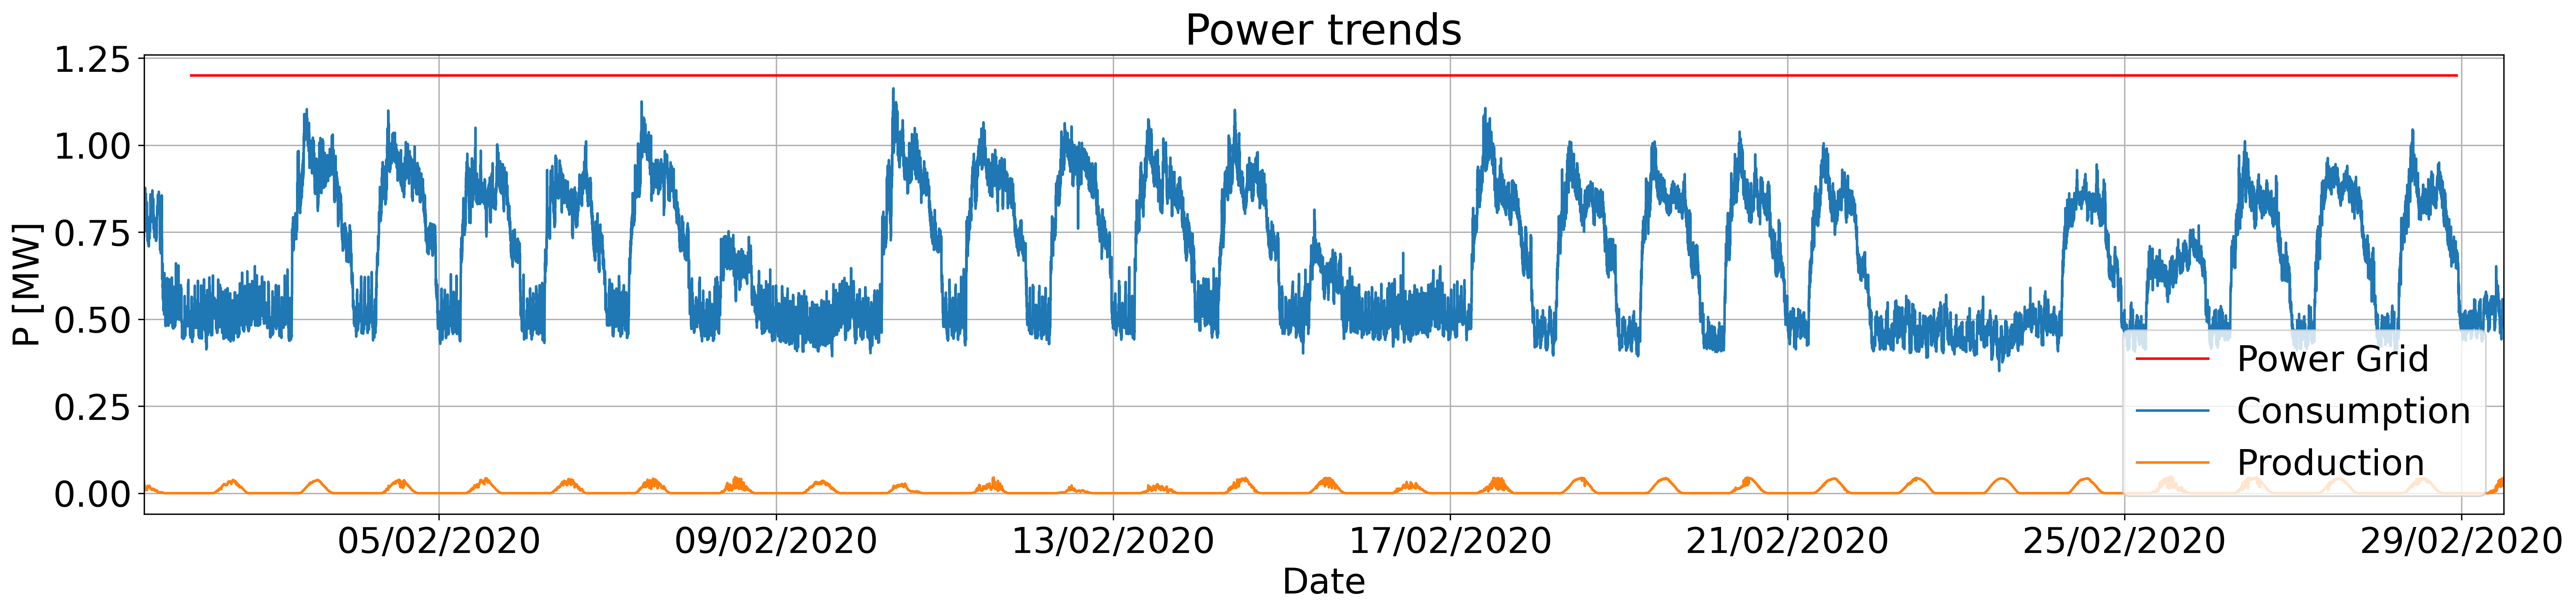
\includegraphics[width=1\linewidth]{Images/Max_cons_prod.png}}
    \subcaptionbox{ \label{available_power}}{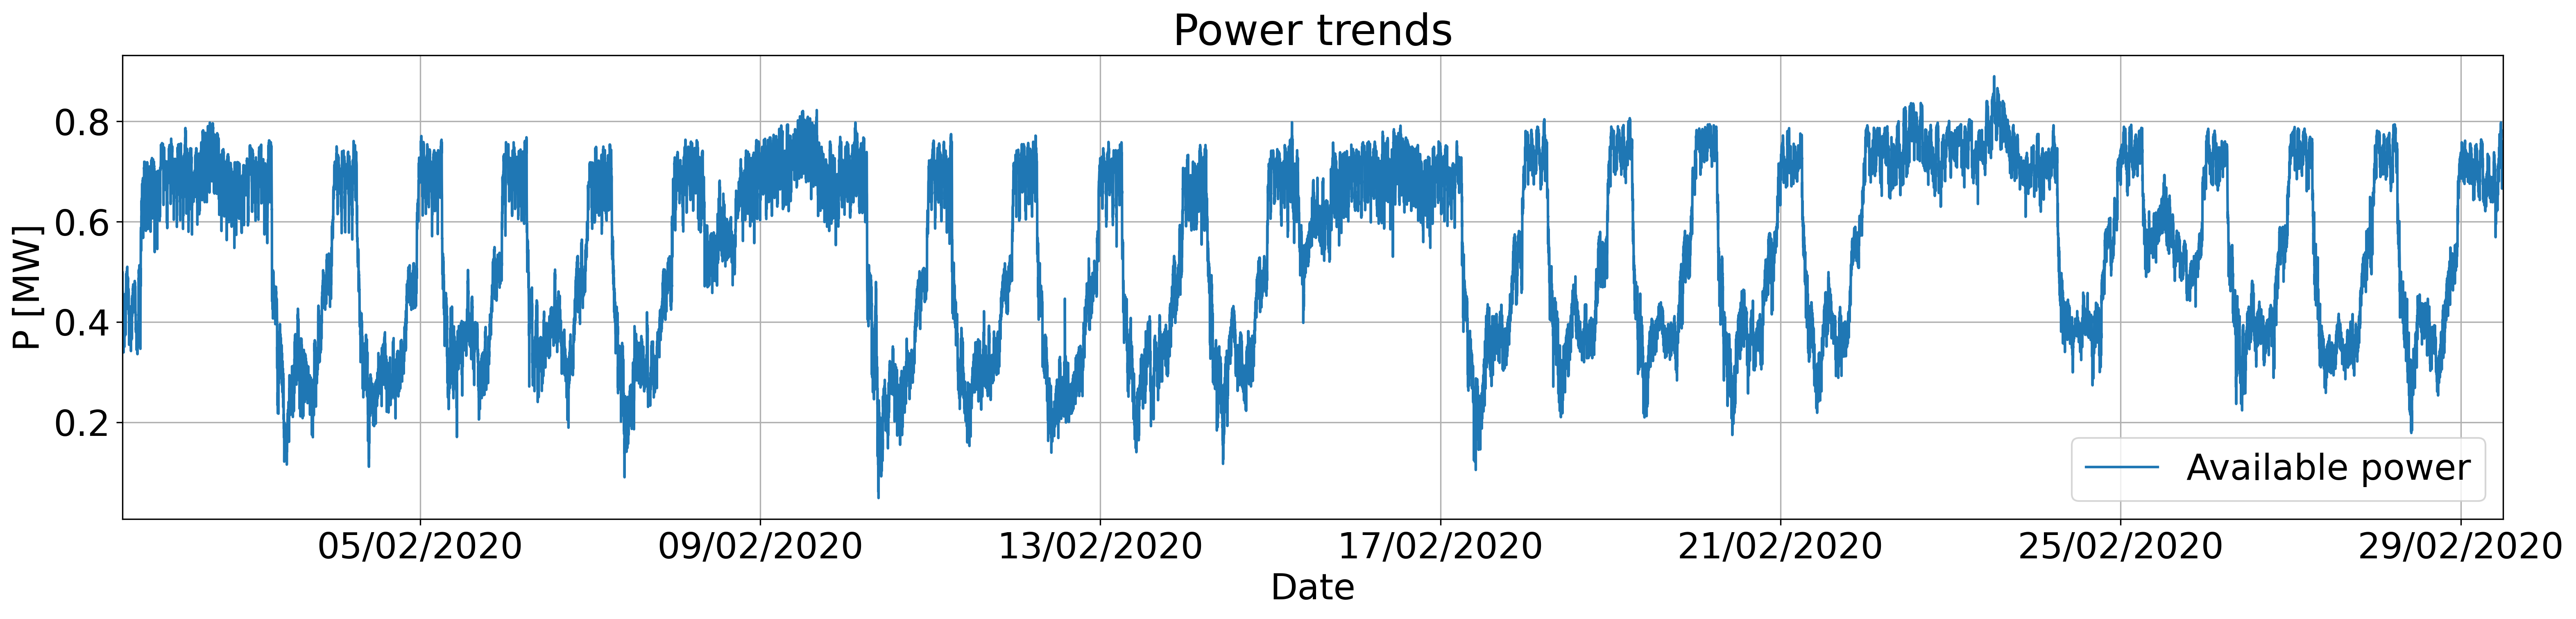
\includegraphics[width=1\linewidth]{Images/Available_power.png}}
    \caption{EDP's building power trends a) grid capacity, consumption and production b) available power.}
\end{figure}


By analyzing Figure \ref{Max_cons_prod}, it can be verified that, compared to the consumption presented by the building, the \ac{PV} panels do not have enough capacity for the building to be self-sustainable, that is, solar power is far from being enough to maintain the regular operation of the building. It can be concluded that the influence of the power generated by the solar panels on the available power of the building is quite reduced. 

The value of the available power is a computed metric, given by:

\begin{equation}
   P_{available} = P_{grid} + P_{solar} - P_{consumption},
   \label{available}
\end{equation}

where $P_{grid}$ is the maximum power that is made available to the building, provided by the electrical grid, which in this particular case is around 1.2 MW, $P_{solar}$ is the active solar power produced by the \ac{PV}, and $P_{consumption}$ denotes the the current power consumption of the building. In Figure \ref{available_power}, the available power profile is shown for the same time interval as Figure \ref{Max_cons_prod}. Like the previous variables, it shows an equally cyclical behavior.


Taking into account all the factors mentioned, it was then decided to choose solution 2, in which the value of the available power is calculated beforehand, and is then used as input for the predictive model. This solution was chosen because it is a simpler architecture and requires less computational capabilities, since the model makes forecasts for only one variable, and not for two. Furthermore, the flexibility offered by forecasting the two variables separately is irrelevant in the context of the problem, since for the proposed objective, it is not necessary to differentiate the consumption forecast from the production forecast. 

\section{Data}\label{chap3:sec:data}

In this section, we describe the datasets used in the development of this work, and also detail the data preprocessing applied to the datasets in order to have the necessary formatting to be used during this experiment.

\subsection{Data description}\label{chap3:subsec:data_description}

In the day to day of a building, there are many factors that influence its consumption and consequently, the available power. In Chapter \ref{chap:background}, some examples of work developed with the objective of predicting the energy consumption of a building were mentioned. In Appendix B, Table \ref{table1}, it is possible to verify that generally, two categories of data are used in this kind of applications, data that concern the behavior of the building, and climatic data that characterizes the surrounding environment of the building.

Regarding the energy behavior of the building, \ac{EDP} provided two different datasets that present information between January 25, 2020 and September 30, 2020, totalling 8 months and 5 days of data, with a granularity of 5 seconds. The first dataset includes historical data concerning the power consumption of the building, and the second dataset includes historical data regarding the solar power production generated by the \ac{PV} panels present in the upper part of the building. It is also relevant to mention that the production data provided showed some gaps, resulting from sensor reading failures. This aspect implies the need for some automatic mechanisms to complete the missing data, which are described below.

Regarding climate data, \ac{FCUL} provided two different datasets that present information between January 25, 2020 and June 15, 2020, totaling 4 months and 21 days of data, with a granularity of 1 minute. The first dataset includes meteorological data of the geographical location of the building, and the second includes data with respect to solar radiation exerted on the geographical location of the building. Neither of the two datasets had temporal flaws.

In Table \ref{table2}, there is a summary of the key points of the available data. The description of the variables for each of the datasets provided can be found in Appendix \ref{chapter:appendixE}, Table \ref{tab:datset_variables}.

\begin{table}[htbp]
  \centering
  \caption{Summary of the datasets used.}
    \begin{tabular}{lr|cccc}
    \toprule
    \multicolumn{2}{c|}{\textbf{Provider}} & \multicolumn{2}{c}{\textbf{EDP}} & \multicolumn{2}{c}{\textbf{FCUL}} \\
    \midrule
    dataset &       & Consumption & Production & Meteorological & Radiation \\
    \# variables &       & 8     & 7     & 21    & 27 \\
    period &       & \multicolumn{2}{c}{8 motnhs and 5 days} & \multicolumn{2}{c}{4 motnhs and 21 days} \\
          & beginning date & \multicolumn{2}{c}{25-01-2020} & \multicolumn{2}{c}{25-01-2020} \\
          & ending date& \multicolumn{2}{c}{30-09-2020} & \multicolumn{2}{c}{15-06-2020} \\
    \# days &       & \multicolumn{2}{c}{249} & \multicolumn{2}{c}{142} \\
    \# samples &       & \multicolumn{2}{c}{4302720} & \multicolumn{2}{c}{2453760} \\
    \end{tabular}%
  \label{table2}%
\end{table}%


As can be seen through the analysis of Table \ref{table2}, the data provided do not portray the same time window nor have the same granularity. It is then necessary to proceed to some data treatment in order to obtain the data in the desired form.

\subsection{Data completion}\label{chap3:subsec:data_completion}

The data manipulation consists of a process in which the data made available is formatted in such a way that it meets the essential criteria to enable its introduction in the models. During the development of the thesis, this was the most time consuming process. The data treatment is an extremely demanding process, which is simplified in the diagram of Figure \ref{datatreatment}.

\begin{figure}[h!]
    \centering
    \begin{center}
    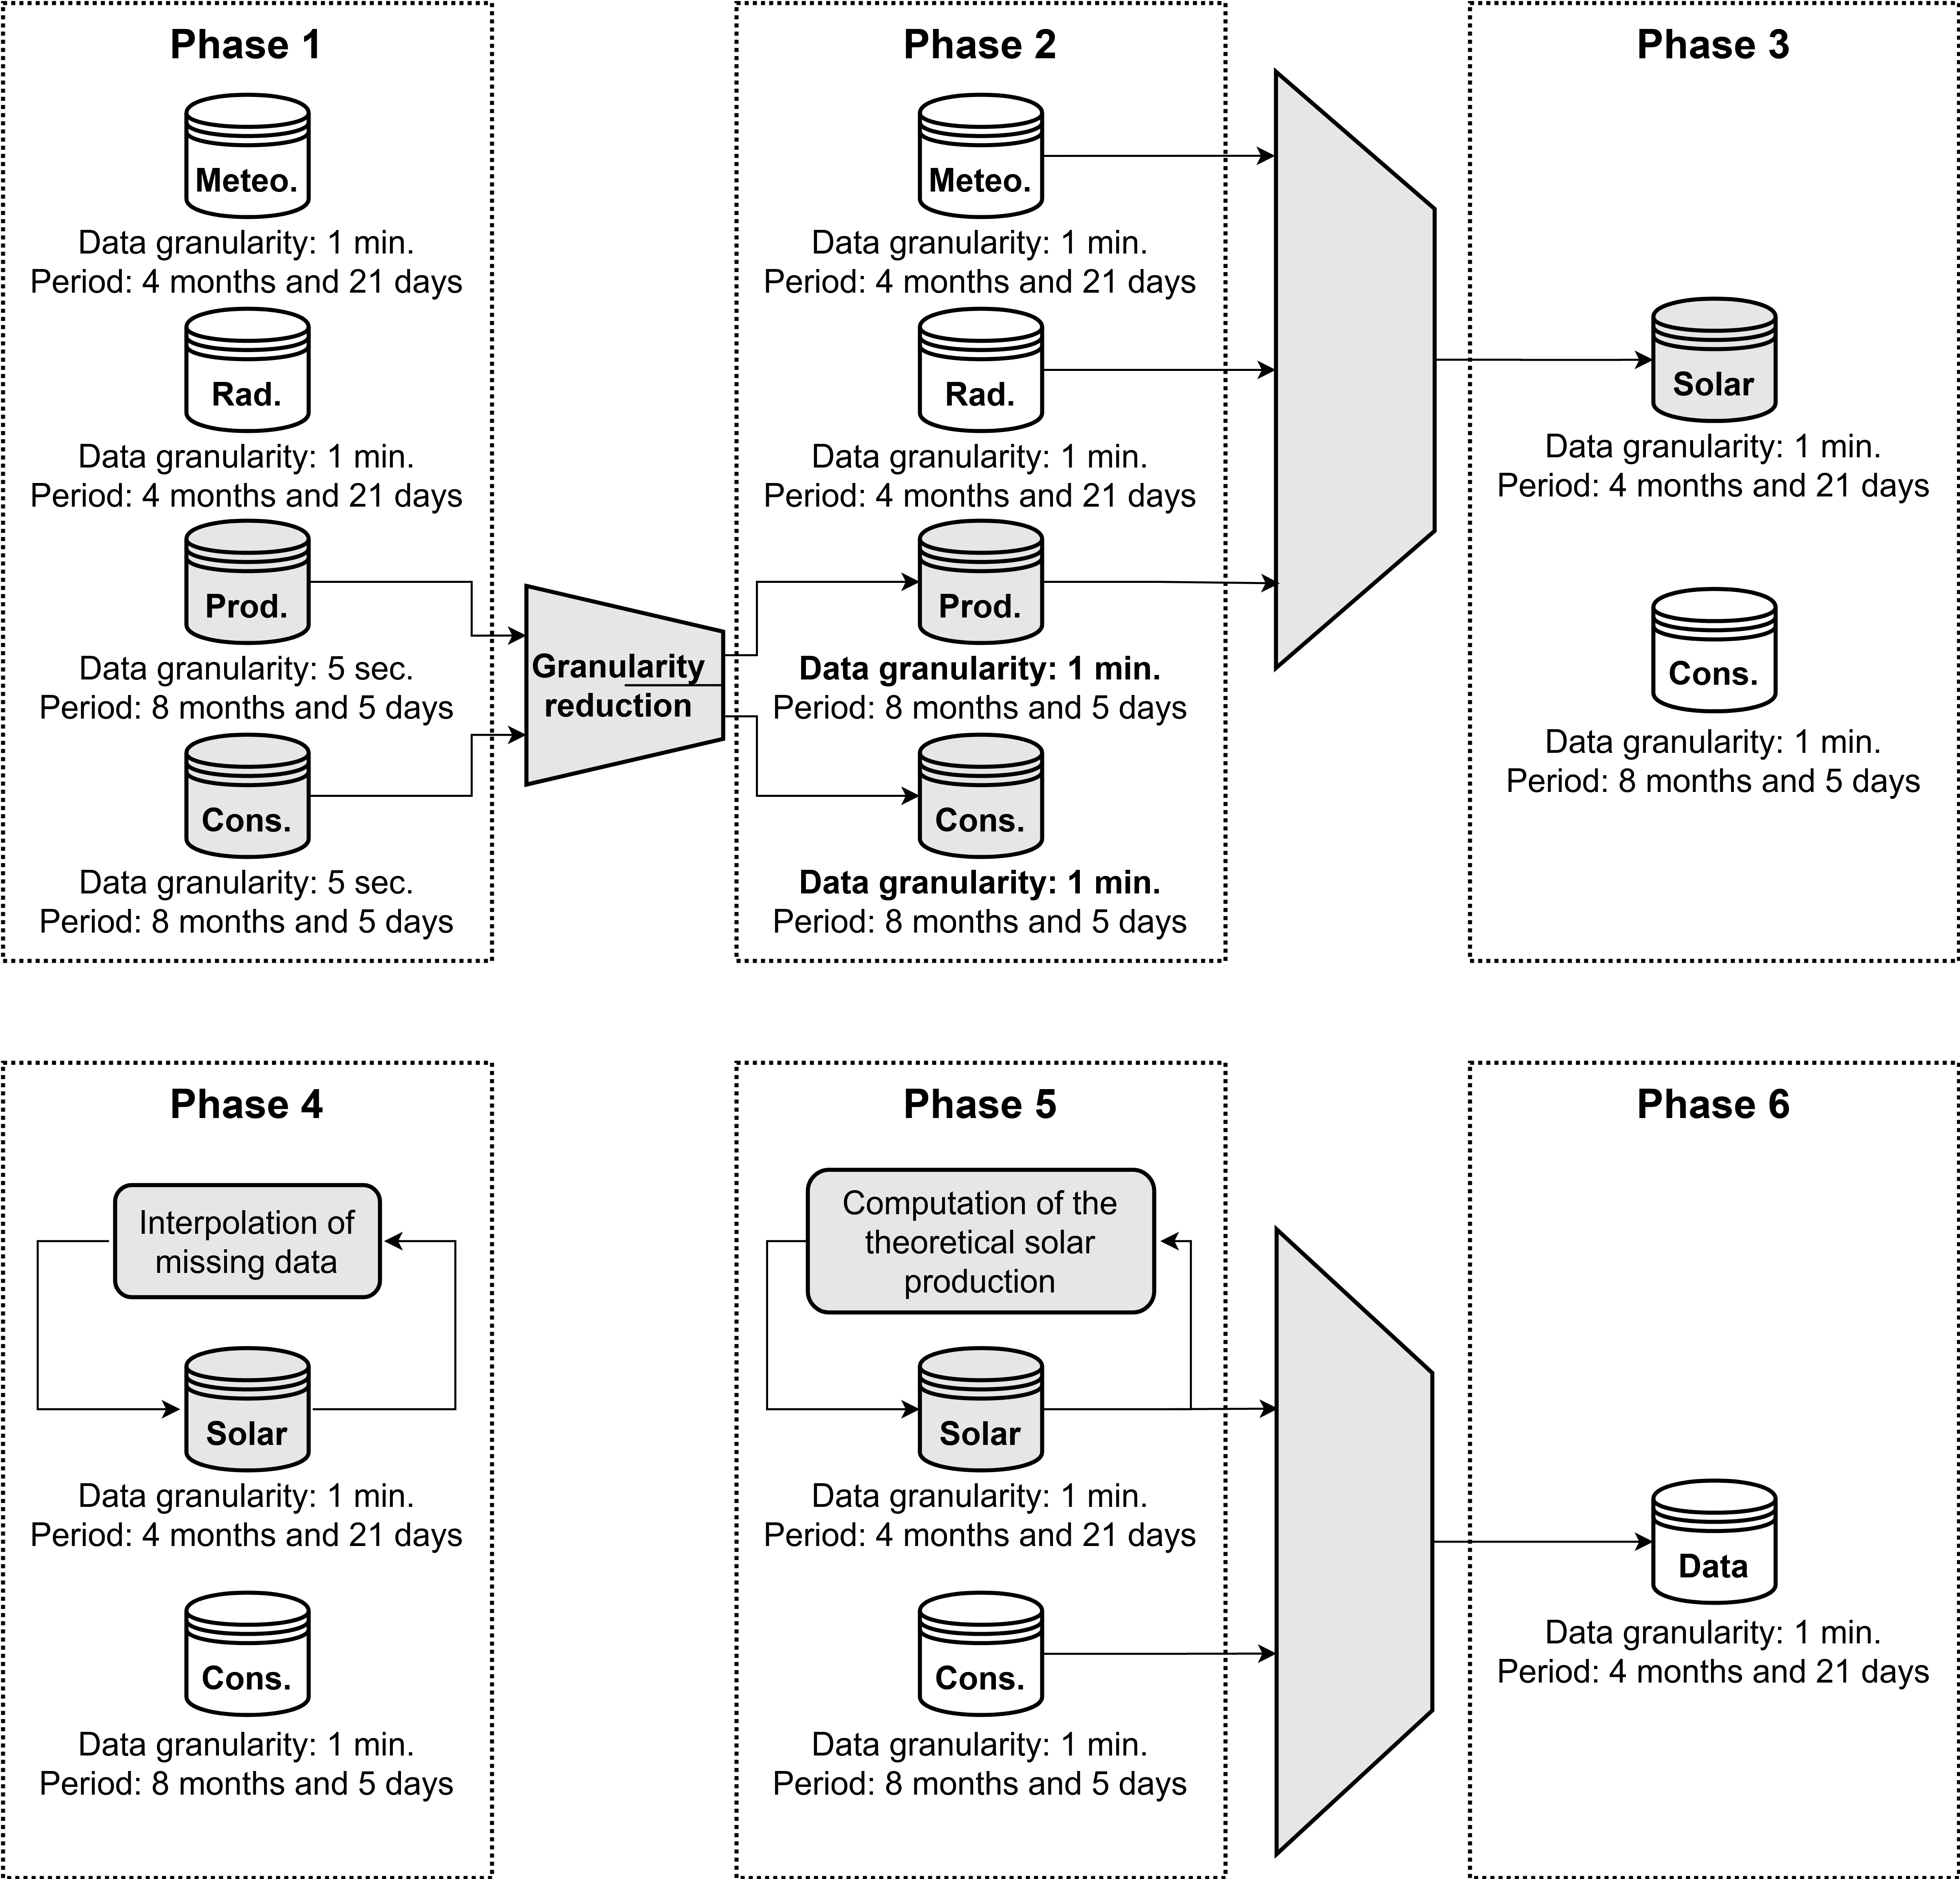
\includegraphics[width=1\textwidth]{Images/Data.png}
    \caption{Data treatment process.}
    \label{datatreatment}
    \end{center}
\end{figure}

In Phase 1, the production data (Prod.) is incomplete due to failure of the system responsible for acquiring and storing this indicator. There is also a difference both in granularity and period available, between the data provided by \ac{EDP} and the data provided by \ac{FCUL}. It is then necessary, first of all, to equal the granularity of all four datasets. In order to do that, a function was applied to reduce the granularity of the production (Prod.) and consumption (Cons.) datasets, forcing the frequency of both datasets to one minute. the  The function applies an arithmetic mean given by 

\begin{equation}
     A={\frac {1}{n}}\sum _{i=1}^{n}a_{i}={\frac {a_{1}+a_{2}+\cdots +a_{n}}{n}},
\label{amean}
\end{equation}

where $A$ represents the value of the final measure with frequency of 1 minute, and $n$ represents the number of nodes between that minute range that will be converted to a single value. We then reached Phase 2, where the four datasets have the same granularity. Then, the datasets corresponding to the meteorological data (Meteo.), radiation data (Rad.) and production data (Prod.) are concatenated. As a result of this process (Phase 3), the dataset (Solar) is formed, which aggregates all the information regarding climate data and solar production data over a period of 4 months and 21 days. The reason behind this phenomenon is that all the production days for which there is no direct correspondence in the meteorological data (Meteo.) and radiation data (Rad.) datasets are dropped. 

As mentioned before, the data regarding the solar production (Prod.) presented some temporal flaws. In order to solve the problem, two solutions were found. For time gaps of less than 30 minutes (Phase 4), a quadratic interpolation was applied. As an example, given any three points $(x_0, f(x_0))$, $(x_1, f(x_1))$ and $(x_2, f(x_2))$, the polynomial that interpolates the three points is given by

\begin{equation}
\begin{split}
     & f_2(x)=b_0+b1(x-x_0)+b_2(x-x_0)(x-x1),\\
     & where:\\
     & b_0=f(x_0),\\
     & b_1=f[x_0,x_1]=\frac{f(x_1)-f(x_0)}{x_1-x_0},\\
     & b_2=f[x_0,x_1,x_2]=\frac{\frac{f(x_2)-f(x_1)}{x_2-x_1}-\frac{f(x_1)-f(x_0)}{x_1-x_0}}{x_2-x_0}.\\
\end{split}
\label{poly}
\end{equation}

In order to exemplify the evolution of the incomplete dataset construction, in the graph of Figure \ref{int0} we can observe the solar power generated measured by the sensors on February 24, 2020. In red, is the portion of data that were measured, corresponding to the Solar dataset in Phase 3 represented in Figure \ref{datatreatment}. After the interpolation, to the original dataset are added the points represented in blue, which represent measurement failures of less than 30 minutes, resulting from the interpolation procedure explained before. At the end of Phase 4, the dataset is then composed of the data points represented in blue plus the points represented in red.



\begin{figure}[h!]
    \centering
    \begin{center}
    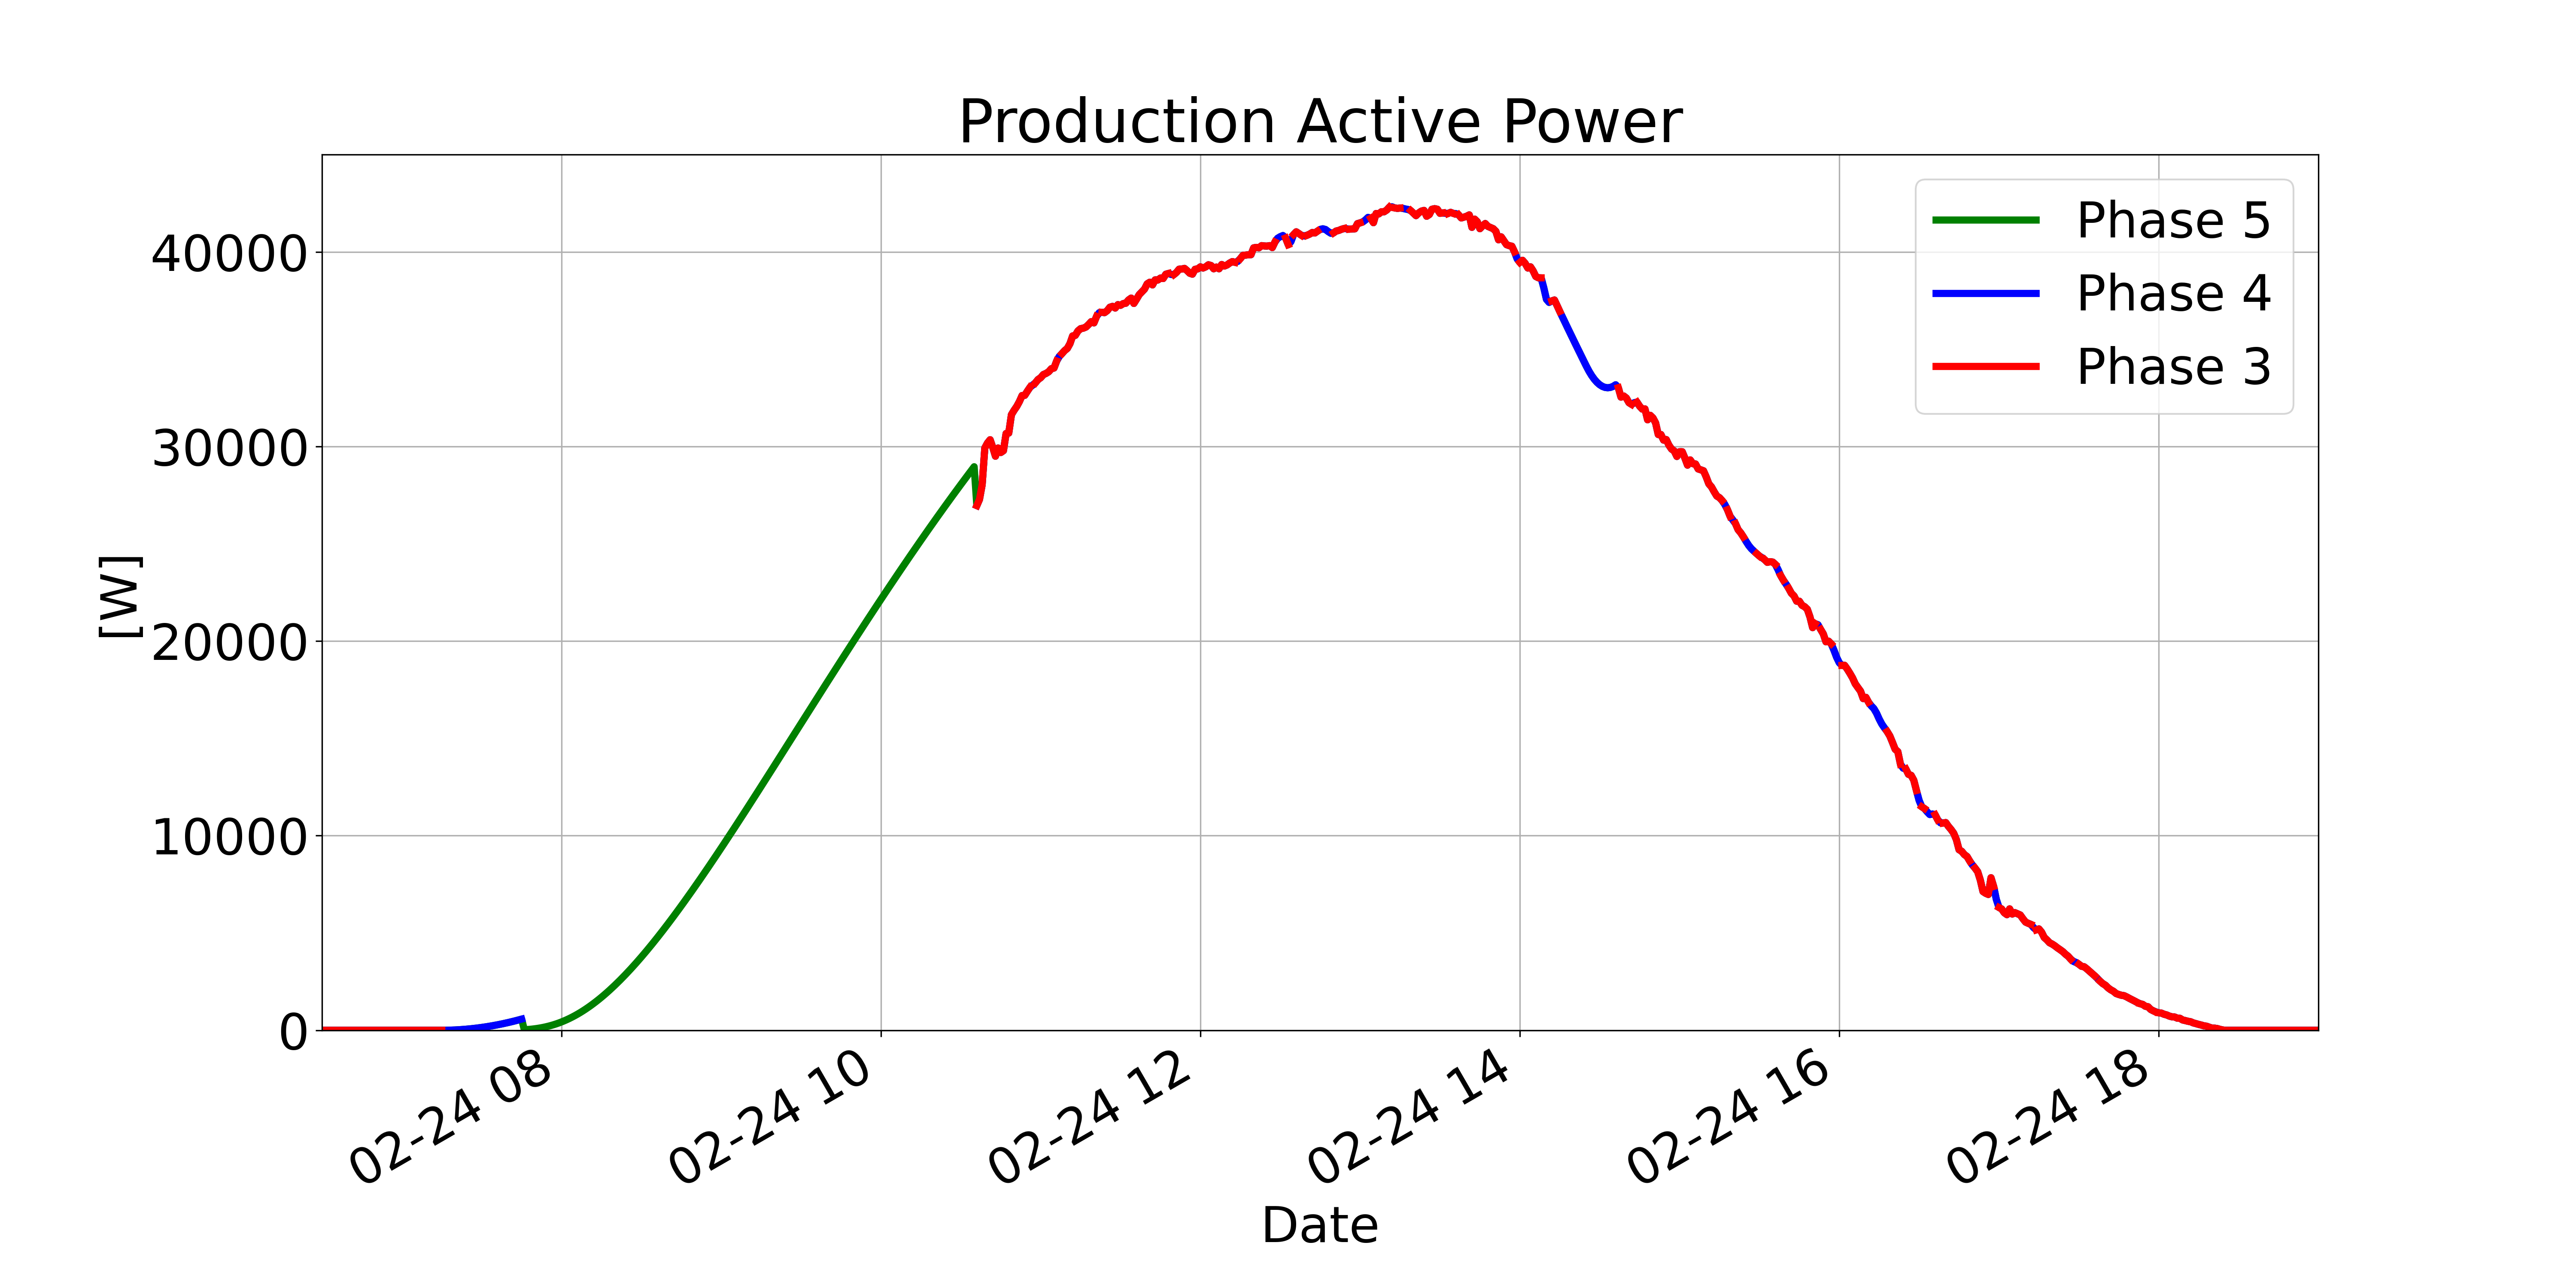
\includegraphics[width=1\textwidth]{Images/int0.png}
    \caption{Data treatment process.}
    \label{int0}
    \end{center}
\end{figure}





For time failures of over 30 minutes, the dataset was completed with theoretically computed values, since the interpolation for large temporal failures does not present the expected behavior.
Based on the equation of the sun's position in the sky throughout the year, the maximum amount of solar insolation on a surface at a particular tilt angle can be calculated as a function of latitude and day of the year\cite{solar0}. In order to determine the direct component of solar radiation in $kW/m^2$, one used


\begin{equation}
     I_D = I_0*0.7^{(AM^{0.678})},
\label{solar}
\end{equation}

where $I_0$ is the solar intensity external to the Earth's atmosphere that is approximately $1.353 kW/m^2$, $0.7$ represents the overall attenuation of the atmosphere, $AM = \frac{1}{cos\theta}$ is the airmass and $\theta$ is the zenith angle (90° minus the altitude) of the sun. This formula produces an optimal result when there are no clouds. Multiplying the resulting value by the total area of panels in the building and taking into account their positioning efficiency, a theoretical value of power generated by the \ac{PV} panels is obtained, in an ideal scenario. In Phase 5, all missing readings were replaced by the calculated theoretical value, as can be seen in Figure \ref{int0} in green. This way, the Solar dataset was completed. It is possible to verify that the point of change between the theoretical data (the green one) and the original data (the red one) is somewhat sudden, because the green signal considers an ideal scenario and the red signal represents real measurements (affected by clouds, cranes, etc.) The sum of the green, blue and red signals, result in a complete signal for the solar active power generated by the \ac{PV} panels.


In Phase 6 the Solar and Cons. datasets were concatenated, thus reducing the dataset time interval to a final result of 4 months and 21 days.

\subsection{Data partition}\label{chap3:subsec:data_partition}

In order to study a certain algorithm, it is necessary to have access to past data to train the model and then evaluate its performance. The the available data is key point when it comes to developing predictive models. Usually, in \ac{ML}, to study a certain model, the dataset should be divided into three sets as can bee seen in Figure \ref{division}. 

\begin{figure}[h!]
    \centering
    \begin{center}
    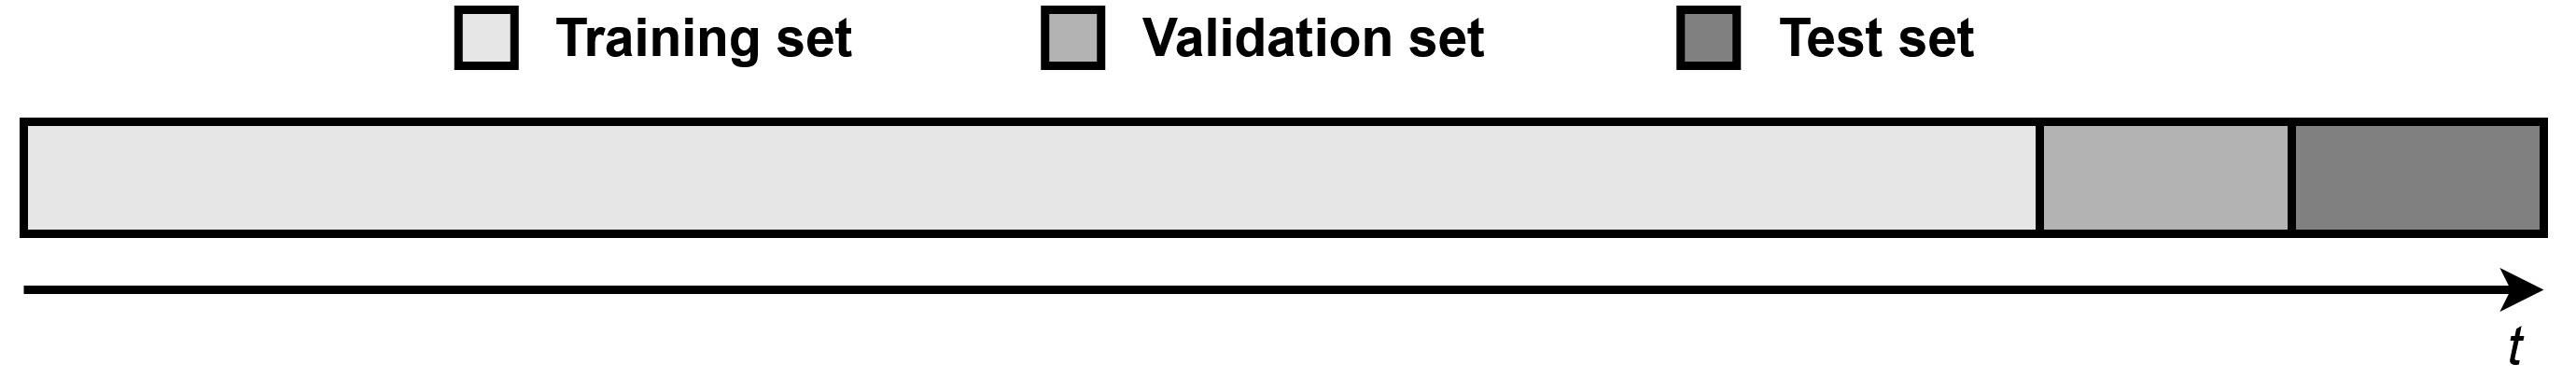
\includegraphics[width=1\textwidth]{Images/division.png}
    \caption{Dataset division.}
    \label{division}
    \end{center}
\end{figure}

The first set is known as a training set, and consists of a dataset used to feed the model with examples in order to fit the hyperparameters, such as the weights of connections between neurons in artificial neural networks. As the name implies, the training set is suitable to train the model, progressively adapting the model to its intended purpose. The second is the validation set, which is responsible for simultaneously continuing to adapt the hyperparameters of the model, while providing an unbiased evaluation of the model fit. In addition to that, it can be used for regularization, as will be explored in a later section. Finally, the test set is an independent dataset of the two previous ones, which has the main objective to evaluate in an unbiased way the performance of the model in unseen data (data that was not used neither in the training process, nor in the validation process). 

One way to use the available dataset to evaluate the proposed models would be to simply apply the standard training-validation-testing division to the entire dataset available, but this strategy would be a poor way to use the small amount of data available. Typically, to evaluate machine learning models on a very limited time interval, k-fold cross-validation is used. This methodology consists, in the first place, in splitting the dataset into K folds.The higher the K value, the less biased the model is, but on the other hand, small folds (large value for K) can lead to errors due to lack of data, so one should choose the K value based on the data available for the specific application. Secondly, the model is trained in K-1 folds and validated on the remaining fold.  This process is repeated until all the K folds have served as the validation set.The average performance on all validation folds shows a more robust result of the model performance evaluation than the standard train-validation-test methodology presented above. However, k-fold cross-validation can present some problems when applied to time-series problems, since one cannot choose random samples and assign them to either the validation set or the training set because it makes no sense to use future values to predict past values. There is a time dependency between observations, and it is essential to preserve this relationship during the entire process. To overcome this barrier, a block cross-validation method was used. This validation methodology is an alternative to k-fold cross-validation that retains the temporal dependence of data. It consists, in the first place, of also separating the data into different blocks. Afterwards, each of these blocks must be split into train and validation data, where the validation data, as in the standard methodology, are temporally subsequent to the training data. After applying this procedure to the different blocks available, an average of the errors presented in the different blocks is then calculated, thus reaching a total error value. 

In Figure \ref{partition}, the reader may find five different sub-datasets, resulting from a division of the main datastet, defined in phase 6, of the section \ref{chap3:subsec:data_completion}. The idea behind this division is to use datasets 1, 2 and 3 block cross-validation, in order to conduct hyperparameter tuning of the different architectures proposed. In a second stage, after tuning the hyperprameters in each of the blocks, one moves on to the test phase, in which the model to be tested, already with the hyperparameters defined, is retrained throughout dataset 4 and tested in the test set.

\begin{figure}[h!]
    \centering
    \begin{center}
    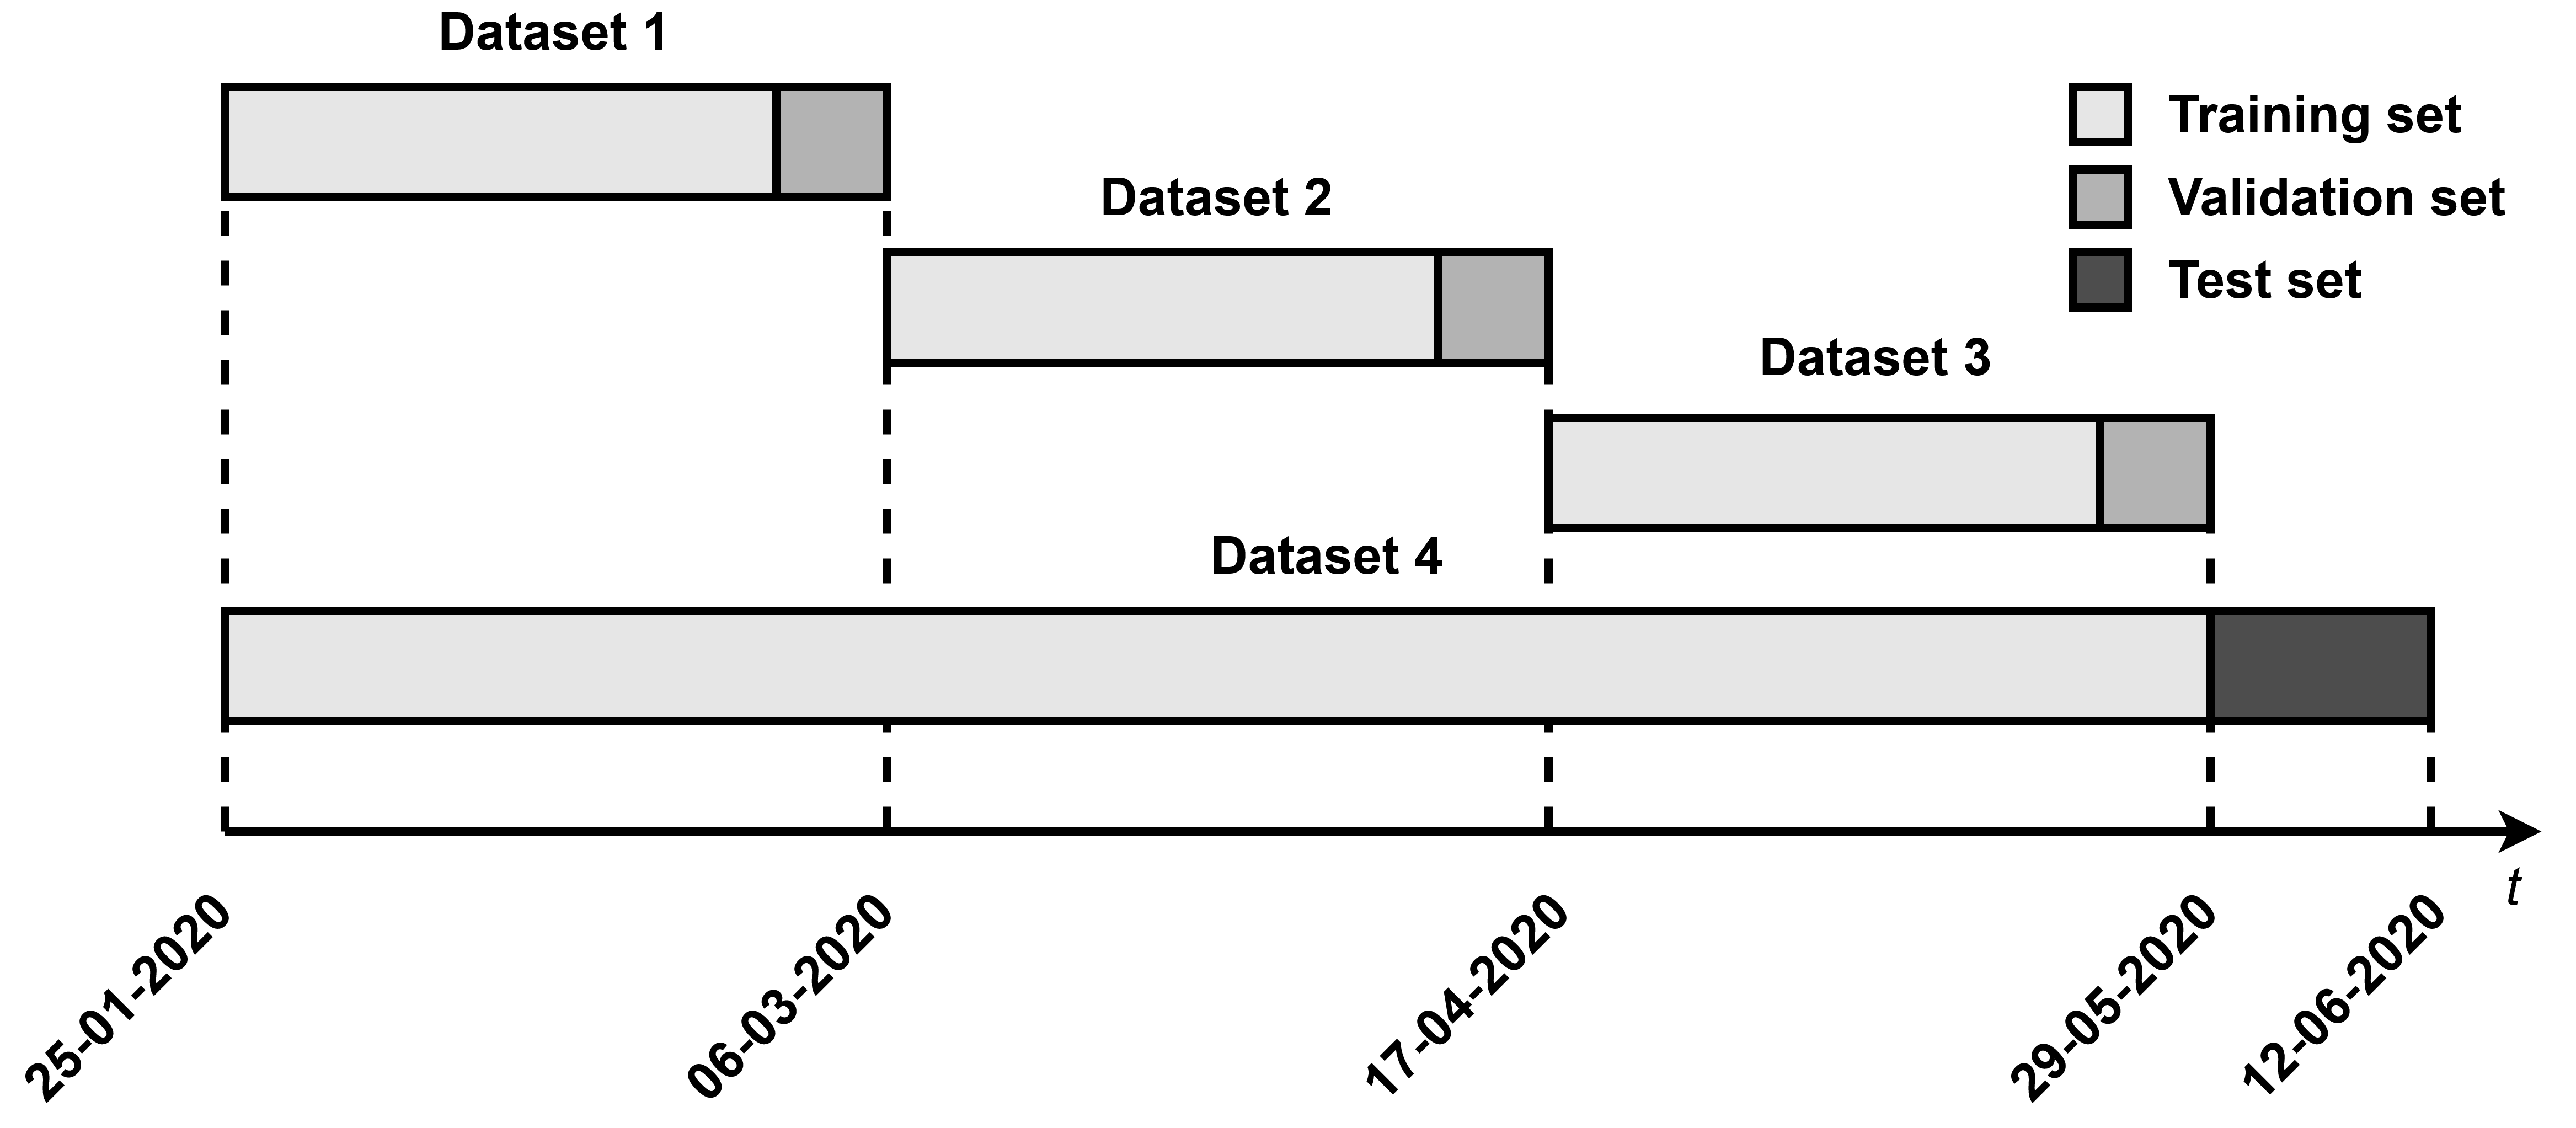
\includegraphics[width=1\textwidth]{Images/data_partition.png}
    \caption{Data partition diagram.}
    \label{partition}
    \end{center}
\end{figure}

The standard approach would be to split dataset 4 in training, validation and testing, but aplying Block cross-validation to to this specific case, consists of dividing the training set in a fixed number of blocks (the number of blocks chosen was 3), and perform training and validation on these blocks.
Datesets 1, 2 and 3 feature five weeks of training and one week of validation. The performance evaluation of the models is then given by the average of the performance in each of these blocks i.e., the error of the models is given by

\begin{equation}
     Model\ error =\frac {1}{k}\ \sum_{i=1}^k Error_{di},
\label{err_av}
\end{equation}

where $Model\ error$ represents the final model error, and $Error_{di}$ represents the error that the model presented while performing in dataset $i$, and $k$ represents the number of datasets used.
In this specific case, the validation error for each model is given by

\begin{equation}
     Model\ error =\frac {1}{3}\ (Error_{d1} + Error_{d2} + Error_{d3}).
\label{err_av}
\end{equation}

The great advantage of using this method is the reduction of the influence of random errors in the selection of the best model. In other words, by performing an average of 3 different sets, the robustness of the choice process is increased since different scenarios are considered and the best model is the one that performs well on average for all of them.

%In a second phase, the models with the best results in the validation data set will be trained again throughout dataset 4 and tested in dataset 5. The predictions resulting from the best models in this test phase (dataset 5), will be used as input for a \ac{DenseNet}, where they will be used as training and validation data. This way, a stacked ensemble model is then constructed, which uses data resulting from the forecasts of all the finalist models to produce a final forecast. This model will then be trained throughout dataset 5 and tested on the test dataset, where its performance will be compared with the individual performance of the finalist models, trained on dataset 4 and tested also on the test dataset. Finally, the dataset 6, represents the entire dataset and presents 18 weeks.

\subsection{Data shifting}\label{chap3:subsec:data_shifting}

While designing a predictive model, the training process is critical so that the model can learn from the data supplied to it. In a time series problem, it would not make sense for the input data to be of the same instant as the output data. When one wants to determine a future value based on current conditions, one needs to train the model to use the input data of the current instant to predict the output data of a future instant. It is then necessary to apply a shift to the output data so that training the model builds a predictive logic. If this shift wasn't applied, one would be training the model to, based on the current instant data, determine the output data of the current instant, and that is not what is intended. As it is already known, one of the main objectives of this thesis is to forecast the available power of the building in 5, 10 and 15 minutes. To do that, it is then necessary that the model can perform 3 forecasts, one for each of these scenarios. Consequently, it is also necessary to apply 3 different shifts to the training data. In Figure \ref{shifting}, the reader can find a graphical representation of the performed procedure.


\begin{figure}[h!]
    \centering
    \begin{center}
    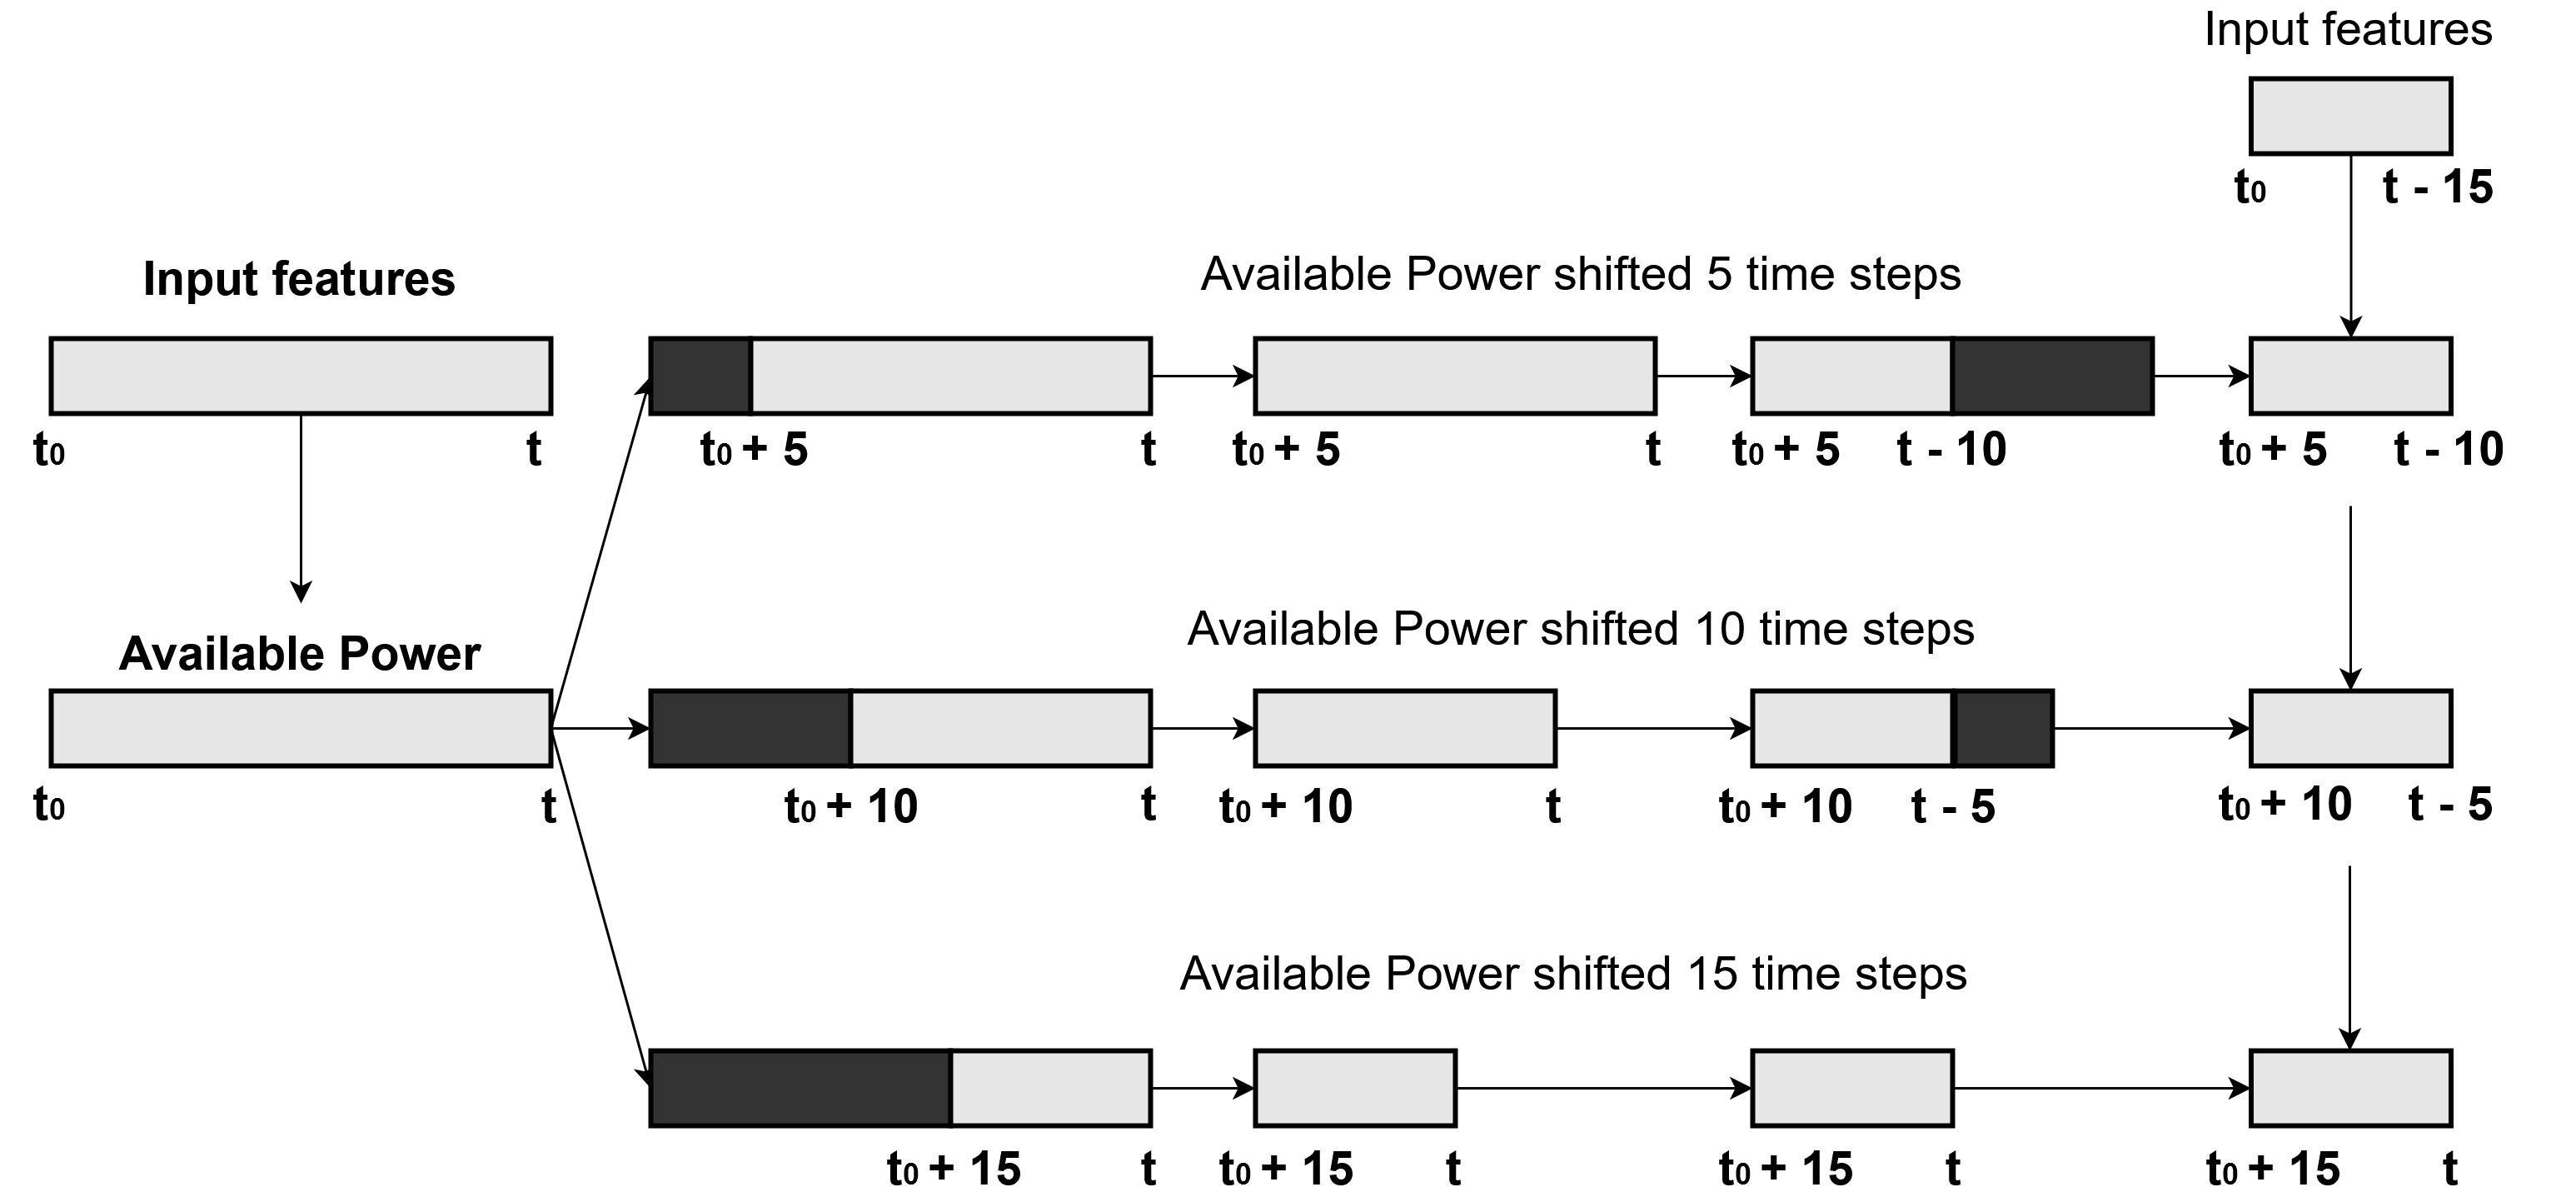
\includegraphics[width=1\textwidth]{Images/Data Shift.png}
    \caption{Data shifting procedure.}
    \label{shifting}
    \end{center}
\end{figure}

In a first instance, one has the data set that corresponds to the features identified as the input features of the model. For the initial scenario, the features of a given instant $t_i$, have a direct match with a value of Available Power of the output variables for the same instant $t_i$.  Then the transformation process begins, where the output variables will be shifted 5, 10 and 15 time-steps. 

The data vector of Available Power is copied originating three identical vectors. In the first step, the 5, 10 and 15 first measurements of each Available Power vector are removed, originating the output vectors with the ranges $[t_0 + 5, t]$, $[t_0 + 10, t]$, $[t_0 + 15, t]$ respectively. At this time each set of input features already presents a match of Available Power in 5, 10 and 15 minutes, but the output vectors present different dimensions as one would expect. In order to have output vectors with the same dimension, the size of the three vectors is limited to the size of the smallest, as well as the set of input features. In the last step there is then a set of input features with values in the range $[t_0, t-15]$ and the ranges $[t_0 + 5, t-10]$, $[t_0 + 10, t-5]$ and $[t_0 + 15, t]$ for the Available Power to 5, 10 and 15 minutes, all four vectors with the same dimension. It is now possible to train the model for the three proposed cases. It should be noted that although there is a reduction in the dataset dimension, this reduction is derisory for the data used. There is a loss of 15 time-steps of data in this whole process. Since the total dataset contains a total of 201542 time-steps, the elimination of these 15 time-steps corresponds to a loss of only 0.0074$\%$ of the information.

\subsection{Feature selection}\label{chap3:subsec:feature_selection}

Although a total of 63 different features have been made available for the development of this work (Appendix \ref{chapter:appendixE}, Table \ref{tab:available_variables}), it is necessary to select which features to use in the development of a \ac{ML} model. Besides the 63 features provided by \ac{EDP} and \ac{FCUL}, 7 other features were also selected, which are listed in Appendix \ref{chapter:appendixE}, Table \ref{tab:computed_variables}. These new features concern calendar metrics such as $hour$, $day\_of\_week$, $day\_of\_month$, $month$ and $holiday$ (a binary indicator that states whether the day in question is a national holiday or not), and also concern calculated metrics such as $AvailablePower$, whose calculation is detailed in section \ref{chap3:sec:variable_to_predict}, and the $TheorethicalValue$, which concerns the theoretical value of the power generated by the \ac{PV} panels, detailed in the section \ref{chap3:subsec:data_completion}. 

A high number of features implies a high complexity of the system architecture. Even though all these features contribute in some way to enrich the past information available, it is important to limit the number of features used. It is then necessary to perform a pre-selection of which features are ideal for the system to produce the best possible results. 

\subsubsection{Dimensionality reduction}


\subsubsection{Correlation Matrix}

From the 70, a set of 16 features that were considered useful in predicting the available power in the building was then pre-selected. 

The criteria used for this selection of of meteorological and radiation data, included selecting unique features that were directly associated with the temperature or solar radiation of the surrounding environment, since, as was verified in section \ref{chap3:sec:building}, the energy consumption of the building is directly linked to the outside temperature and weather conditions. Metrics related to atmospheric pressure and humidity were discarded. Regarding the building, the metrics that refer to the power produced and the power consumed in were selected, but only the final metrics, that is, the three-phase currents and voltages were eliminated since it is from them that the value of power consumed and produced are obtained. As these two variables are also measured, the use of currents and voltages is then discarded. All 7 metrics that relate to the schedule and calculations performed, were also considered. 

It was then necessary to evaluate these 16 pre-selected features. Therefore, the correlation matrix between each of the 16 features was computed. In Figure \ref{corr}, one can then observe the correlation matrix, where the correlations between all the 16 pre-selected features are represented. The value of the correlation is present in the [-1, 1] range, where -1 means that the features present a perfect negative correlation, 0 means that there is no correlation between them, and 1 means that there is perfect positive correlation between the two features. 


\begin{figure}[h!]
    \centering
    \begin{center}
    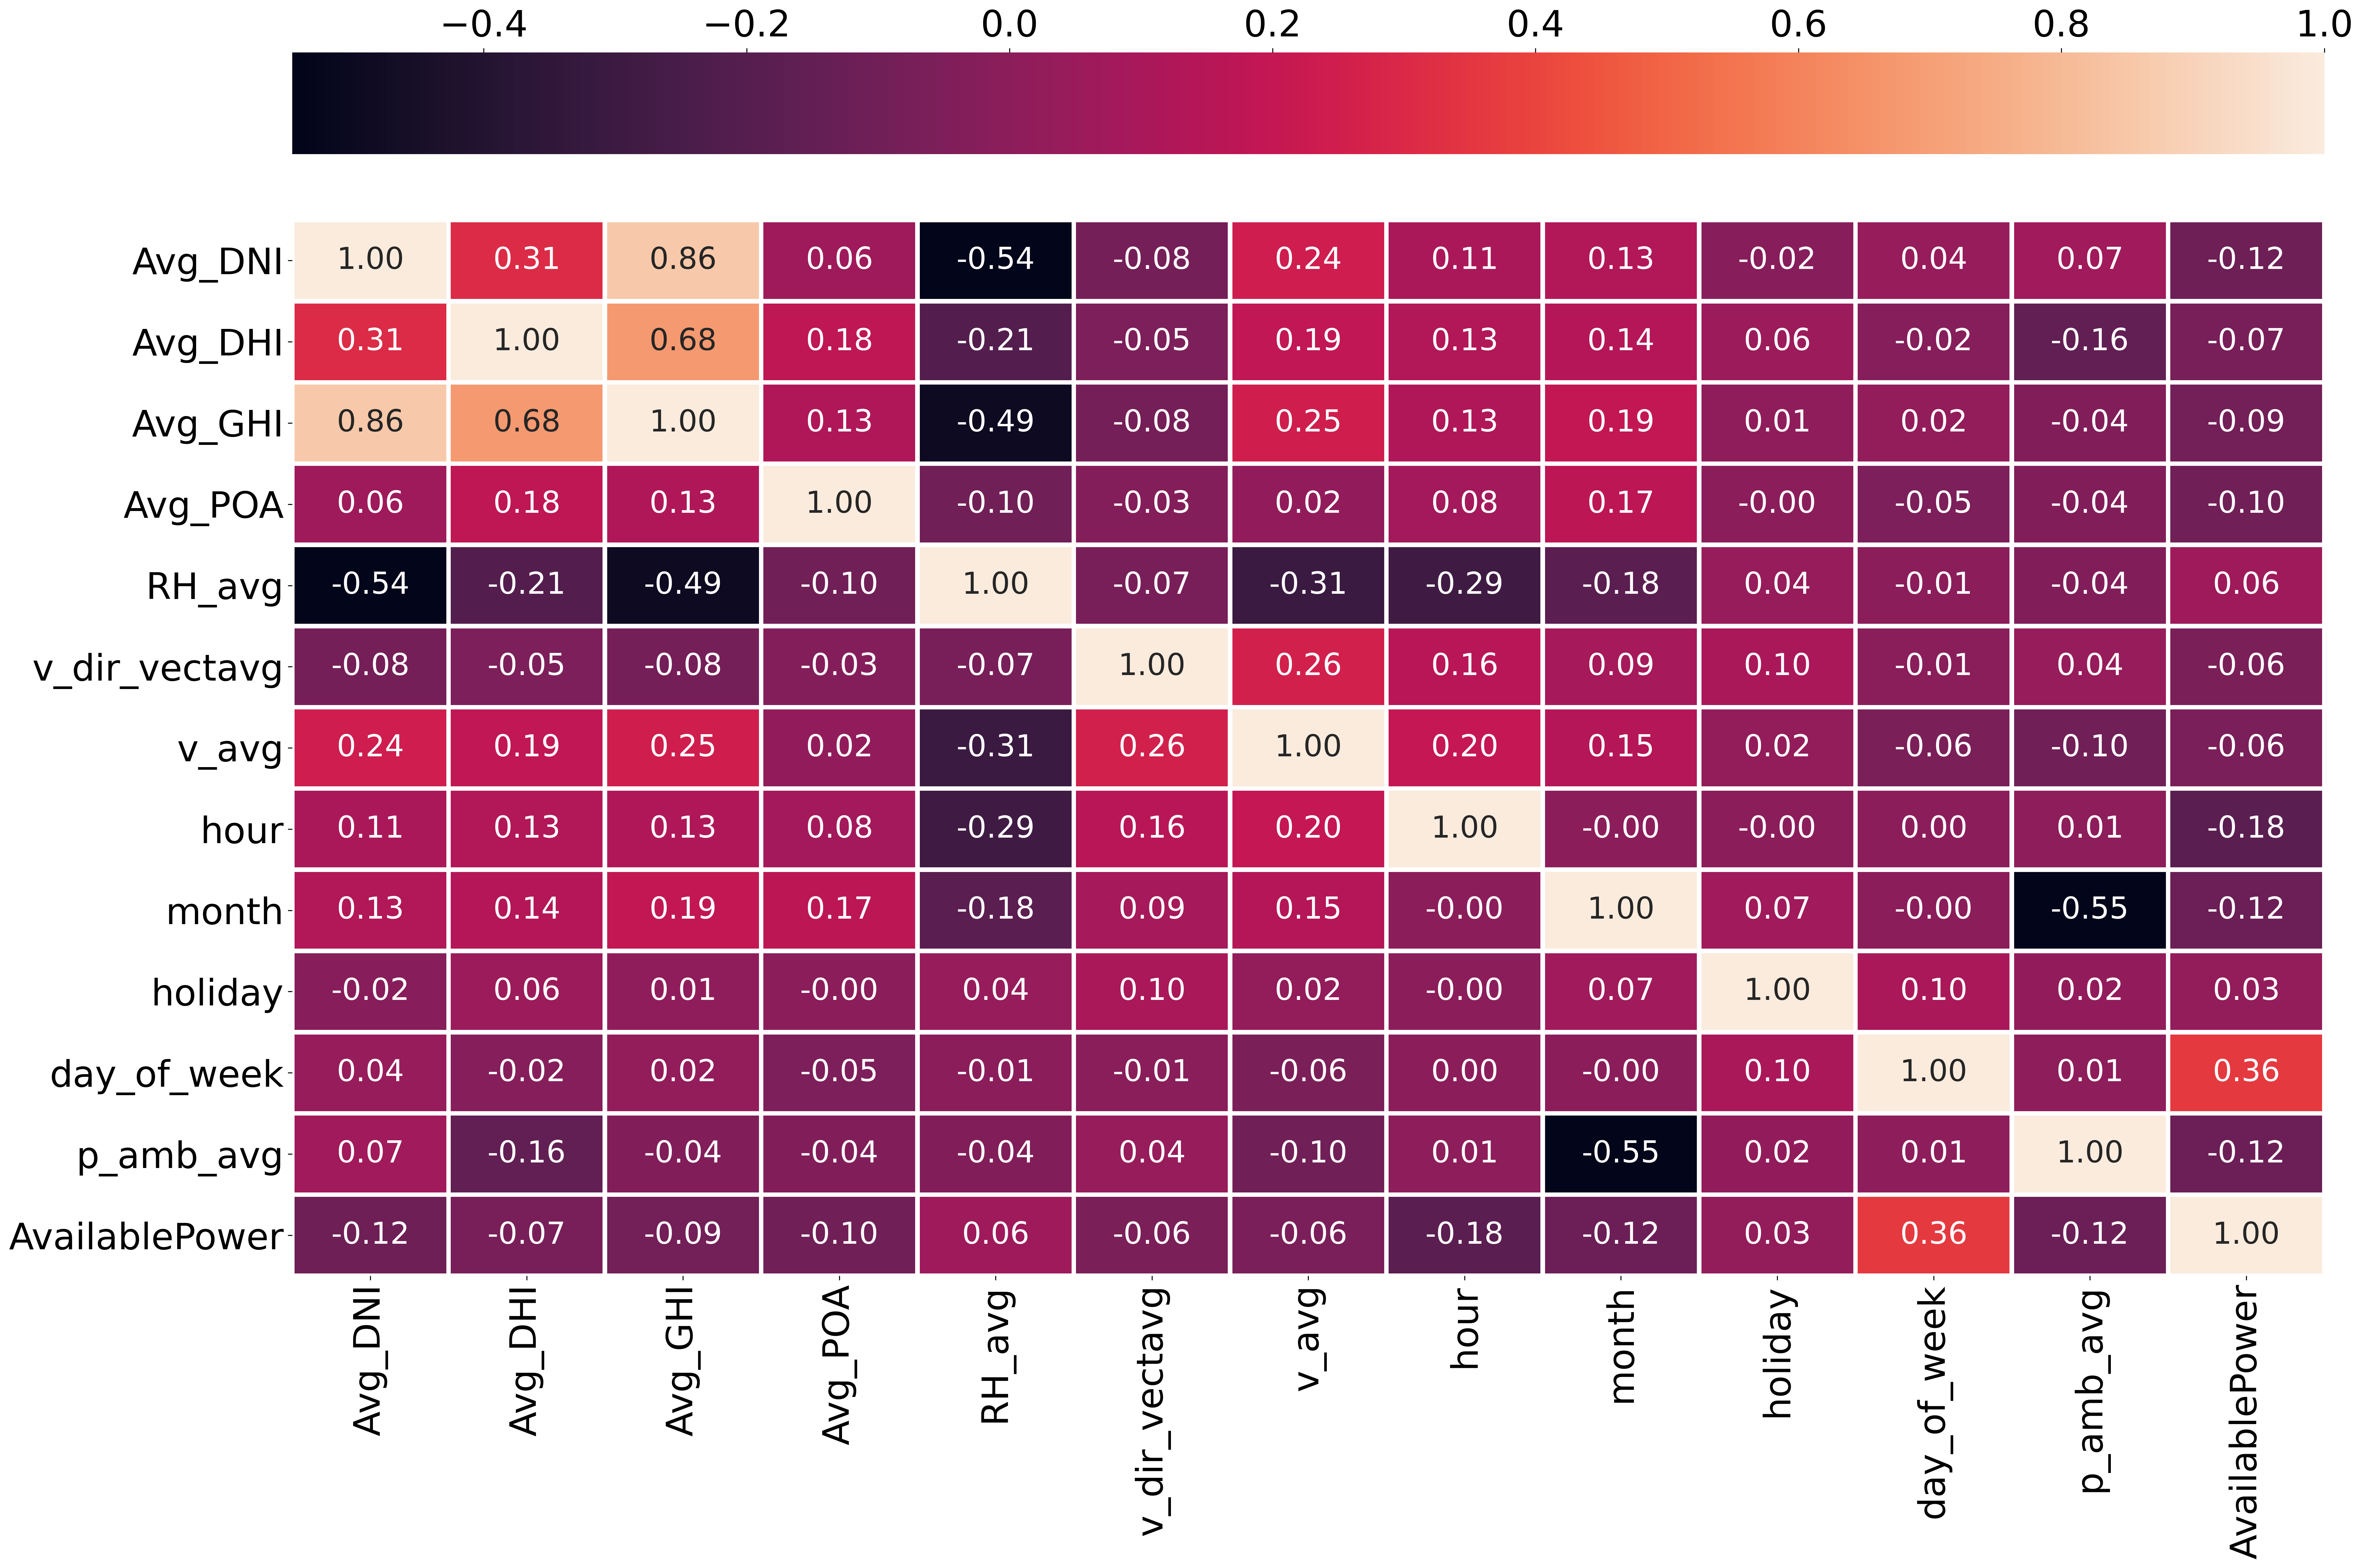
\includegraphics[width=1\textwidth]{Images/corr1.PNG}
    \caption{Feature correlation matrix.}
    \label{corr}
    \end{center}
\end{figure}


The aim of computing this matrix is to identify features that present a perfect or almost perfect correlation between them, both positively and negatively. A perfect correlation between two features means that one can be deduced from the other, that is, the relevance of the two features for the construction of the forecasting system is the same, so one of the features can be eliminated. Using features that present a perfect correlation, one can incur in multicollinearity \cite{multicollinearity}.

After evaluating the projected correlation matrix, it was decided to start to eliminate the features that present an almost perfect correlation, both negative and positive. Starting with positive correlation, S represents the complex power consumed and P the real power consumed, which means that the two values only differ in the imaginary component. Since S does not have an imaginary component, S and P have the same value. The feature S was then discarded. The Theoretical Value and ActPwr also present a perfect correlation. This happens because, as explained in section \ref{chap3:subsec:data_completion}, the readings of the power generated by \ac{PV} panels (ActPwr) showed a lot of flaws. For a time failure longer than 30 minutes, the ActPwr value (which was null) was replaced by the calculated theoretical value of power generated by \ac{PV} panels. The large correlation is then justified by the fact that there were quite a few time flaws, i.e., most of the ActPwr values are similar to the Theoretical Value. The feature Theoretical Value was also discarded. 



Also, although Theoretical Value and Avg\_GHI present a very high correlation with ActPwr (which is predictable given that the measured ActPwr these two variables were added, as explained in section \ref{chap4:vtp}), we chose to keep these two variables as input features since the correlation is not exactly perfect and can be decisive in certain cases in building a good predictive model. Therefore, the variables chosen for the input of all tested models are: Std\_DHI, Avg\_DHI, Avg\_GHI, Avg\_DNI, Avg\_POA, T\_amb\_avg, Theoretical\ Value, ActPwr, P, hour, day\_of\_month, day\_of\_week, month and holiday. In addition, the variable Available Power given in W has been added as an input feature, resulting in a total of 15 input features and 3 output (Available Power in 5, 10 and 15 minutes).

\section{Proposed model}\label{chap3:sec:proposed_model}

In Chapter \ref{chap:background}, some of the most common models were studied with regard to forecasting power consumption in various types of buildings. As has also been mentioned, data-driven models have been widely used in this type of applications. In this thesis, it was also decided to study a solution composed by one or more data-driven models, since historically they present a better performance and an excellent relation between the need of computational resources used, and the obtained performance.

This problem presents some characteristics that are determinant in the process of choosing the models to be tested. First of all, the data made available for this study, represents a significantly short time period, which means that the use of models as statistical regressions are not ideal to solve this problem. On the other hand, the challenge presented by \ac{EDP} implies a 5, 10 and 15 minute data forecast. This factor implies the use of a fast model that is able to produce different forecasts in a short period of time. This is a problem for \ac{SVM}s/\ac{SVR}s because, as mentioned in \cite{svm3}, \cite{svm2} and \cite{svm5} while producing results with good precision an accuracy, they are slow models for large-scale problems. 

Another model presented in Chapter \ref{chap:background}, were the \ac{DT}s. Although they are simple to apply models, \ac{DT}s have the limitation of not allowing a future value to be computed, but rather a range of values in which the variable to be predicted can be found. Since for this problem the main objective is to obtain specific values of available power, this category of models was not considered in this research.

Although all the mentioned models can produce acceptable results for the proposed work, it was decided to apply different types of artificial neural networks, both architectures with only one \ac{ANN} layer, and architectures with multiple layers implemented simultaneously. The idea is then to test various topologies of \ac{ANN}s, and elaborate a comparative study between the proposed solutions, comparing their performance in different scenarios and conditions.

\subsection{Artificial Neural Networks}\label{chap3:subsec:artificial_neural_networks}

Neural networks have proven extremely efficient in identifying and learning temporal data patterns, many of them quite complex. In chapter \ref{chap:background}, two large families of neural networks were presented, \ac{FFNN}s and \ac{RNN}s. From the different existing architectures within these two categories, two types of layers were selected, \ac{GRU} and \ac{LSTM}, both classified as \ac{RNN}s' layers. In addition, \ac{1D CNN} layers were also tested, which fall under the umbrella of \ac{CNN}. These three different types of layers were tested in multiple arrangements and combined with each other to form multiple neural network architectures.

\subsubsection{Long short-term memory (LSTM)}\label{chap3:subsubsec:lstm}

The first type of configuration considered is the \ac{LSTM}, architecture that fits within the group of \ac{RNN}s, proposed et el. \cite{lstm0} by Hochreiter and Schmidhuber in 1997.
\ac{LSTM}s were invented to fight the vanishing gradient problem that is often identified during the training process of common \ac{ANN}s with gradient-based learning methods and back propagation. In these cases, each of the \ac{ANN}'s weights receives an update proportional to the partial derivative of the error function from the current weight in each iteration of training. The problem is that, in some cases, the gradient becomes smaller and smaller with each iteration, preventing the weight from changing its value. This problem leads to a poor performance of the \ac{ANN}, and can even prevent it from continuing the training process.

To avoid this situation, the \ac{LSTM} units are composed of a cell state, an input gate, an output gate and a forget gate, as can be seen in Figure \ref{lstm}.

The responsibility of the cell state is to trace the dependencies between the elements in the input sequence. 

In first place, the forget gate has the purpose of forgetting information that is no longer useful to the state of the cell. This gate has two inputs, $x_t$ (input at the specific time) and $h_{t-1}$ (output from previous cell) which are multiplied by weight matrices, followed by the addition of the bias. The result of this process is passed through a sigmoid $\sigma$ activation function, which provides a binary output. If for a given cell state the output is 0, the information is forgotten, if the output is 1, the information is retained for future use.

The input gate is responsible for adding useful information to the cell state. First, the information is regulated using the sigmoide function that filters the values to be remembered in a similar way to the forget gate, also having as inputs $h_{t-1}$ and $x_t$. In parallel, a vector is created using the $tanh$ function that has as output a value in the range $ [-1, +1]$, which contains all possible values of $h_{t-1}$ and $x_t$. The values of the vector and the regulated values are then multiplied. 

The output gate's task is to extract useful information from the current cell state to be presented as an output. First, a vector is generated by applying the function tanh to the cell. In parallel, the information from the $h_{t-1}$ and $x_t$ inputs is regulated using the sigmoid function that filters the values to be remembered. The values of the vector and the regulated values are then multiplied to be sent as an output and input to the next cell.

 
\begin{figure}[h!]
    \centering
    \begin{center}
    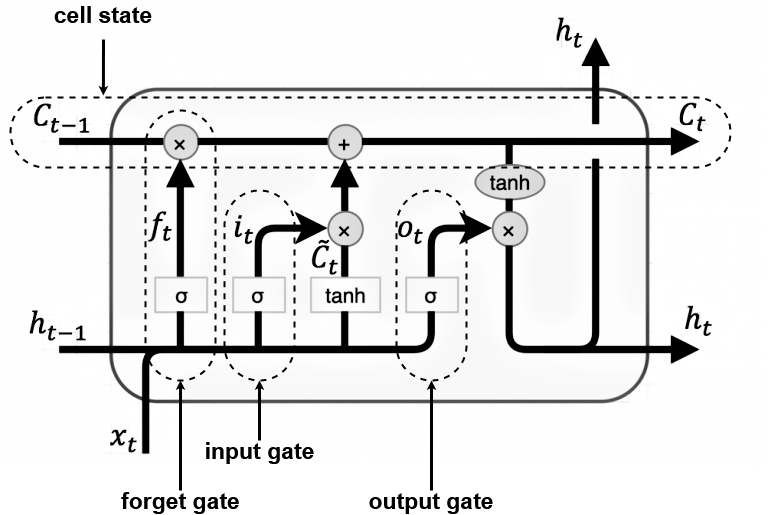
\includegraphics[width=0.6\textwidth]{Images/LSTM_cell_detailed.png}
    \caption{LSTM unit.}
    \label{lstm}
    \end{center}
\end{figure}

The equations that describe the operation of a \ac{LSTM} unit are given by 

\begin{equation}
    \begin{cases} 
        
        f_t=\sigma(W_f.[h_{t-1},x_t] + b_f)\\
        i_t=\sigma(W_i.[h_{t-1},x_t] + b_i)\\
        \widetilde{C}_t = tanh(W_c.[h_{t-1},x_t] + b_C)\\
        C_t=f_t*C_{t-1}+i_t* \widetilde{C}_t\\
        o_t=\sigma(W_o.[h_{t-1},x_t] + b_o)\\
        h_t=ot*tanh(C_t)
        
         
    \end{cases} ,
\end{equation}

where $f_t$ represents the forget, $i_t$ the input gate, $\widetilde{C}_t$ the cell input activation vector, ${C}_t$ the cell state vector, $o_t$ the output gate, $h_t$ the hidden state vector or output vector of the \ac{LSTM} unit. This type of units has then the ability to choose new information that is relevant and delete the past information that is not relevant, maintaining a good functioning, particularly in time series data since there can be lags of undefined length between important events in a time series dataset.

\subsubsection{Gated recurrent unit (GRU)}\label{chap3:subsubsec:gru}

The \ac{GRU} unit is quite similar to \ac{LSTM} with the particular difference that it has no output gate. Introduced in 2014 by Kyunghyun Cho et el. \cite{gru0}, \ac{GRU}s are also part of the \ac{RNN} family. Although they have a similar architecture to \ac{LSTM}s, \ac{GRU}s are simpler models which led to the conclusion that for some cases, where there are smaller datasets and with a lower frequency of repetition, \ac{GRU} architectures perform better than \ac{LSTM} architectures \cite{gru1}, \cite{gru2}.

Compared to \ac{LSTM}s, \ac{GRU}s have no cell state and use the hidden state to transfer information. This architecture has only two gates, a reset gate and an update date, as can be seen in the diagram in Figure \ref{gru}.

The \ac{GRU} structure allows to capture dependencies of large data sequences without discarding information from previous parts of the sequence. This is achieved through its gates, similar to \ac{LSTM}s. These gates are responsible for regulating the information to be kept or discarded at each time interval.

The \ac{GRU}'s ability to maintain a long term memory stems from calculations in the \ac{GRU} unit to produce the hidden state. While \ac{LSTM}s have two different states passed between cells - the cell state, which carries long-term memory, and the hidden state, which carries short-term memory - \ac{GRU}s have only one hidden state transferred between time stages. This hidden state is able to maintain both long term and short term dependencies simultaneously, due to the constraint mechanisms and calculations through which the hidden state and the input data pass.  Like the \ac{LSTM} gates, the gates in the \ac{GRU} are trained to selectively filter out any irrelevant information, keeping what is useful.

These gates essentially produce vectors containing the values 0 or 1 that will be multiplied with the input data and/or hidden state. A value of 0 in the vectors indicates that the corresponding data in the input or hidden state is not important and therefore will be overridden. On the other hand, a value of 1 in the array means that the corresponding data is important and will be used.


\begin{figure}[h!]
    \centering
    \begin{center}
    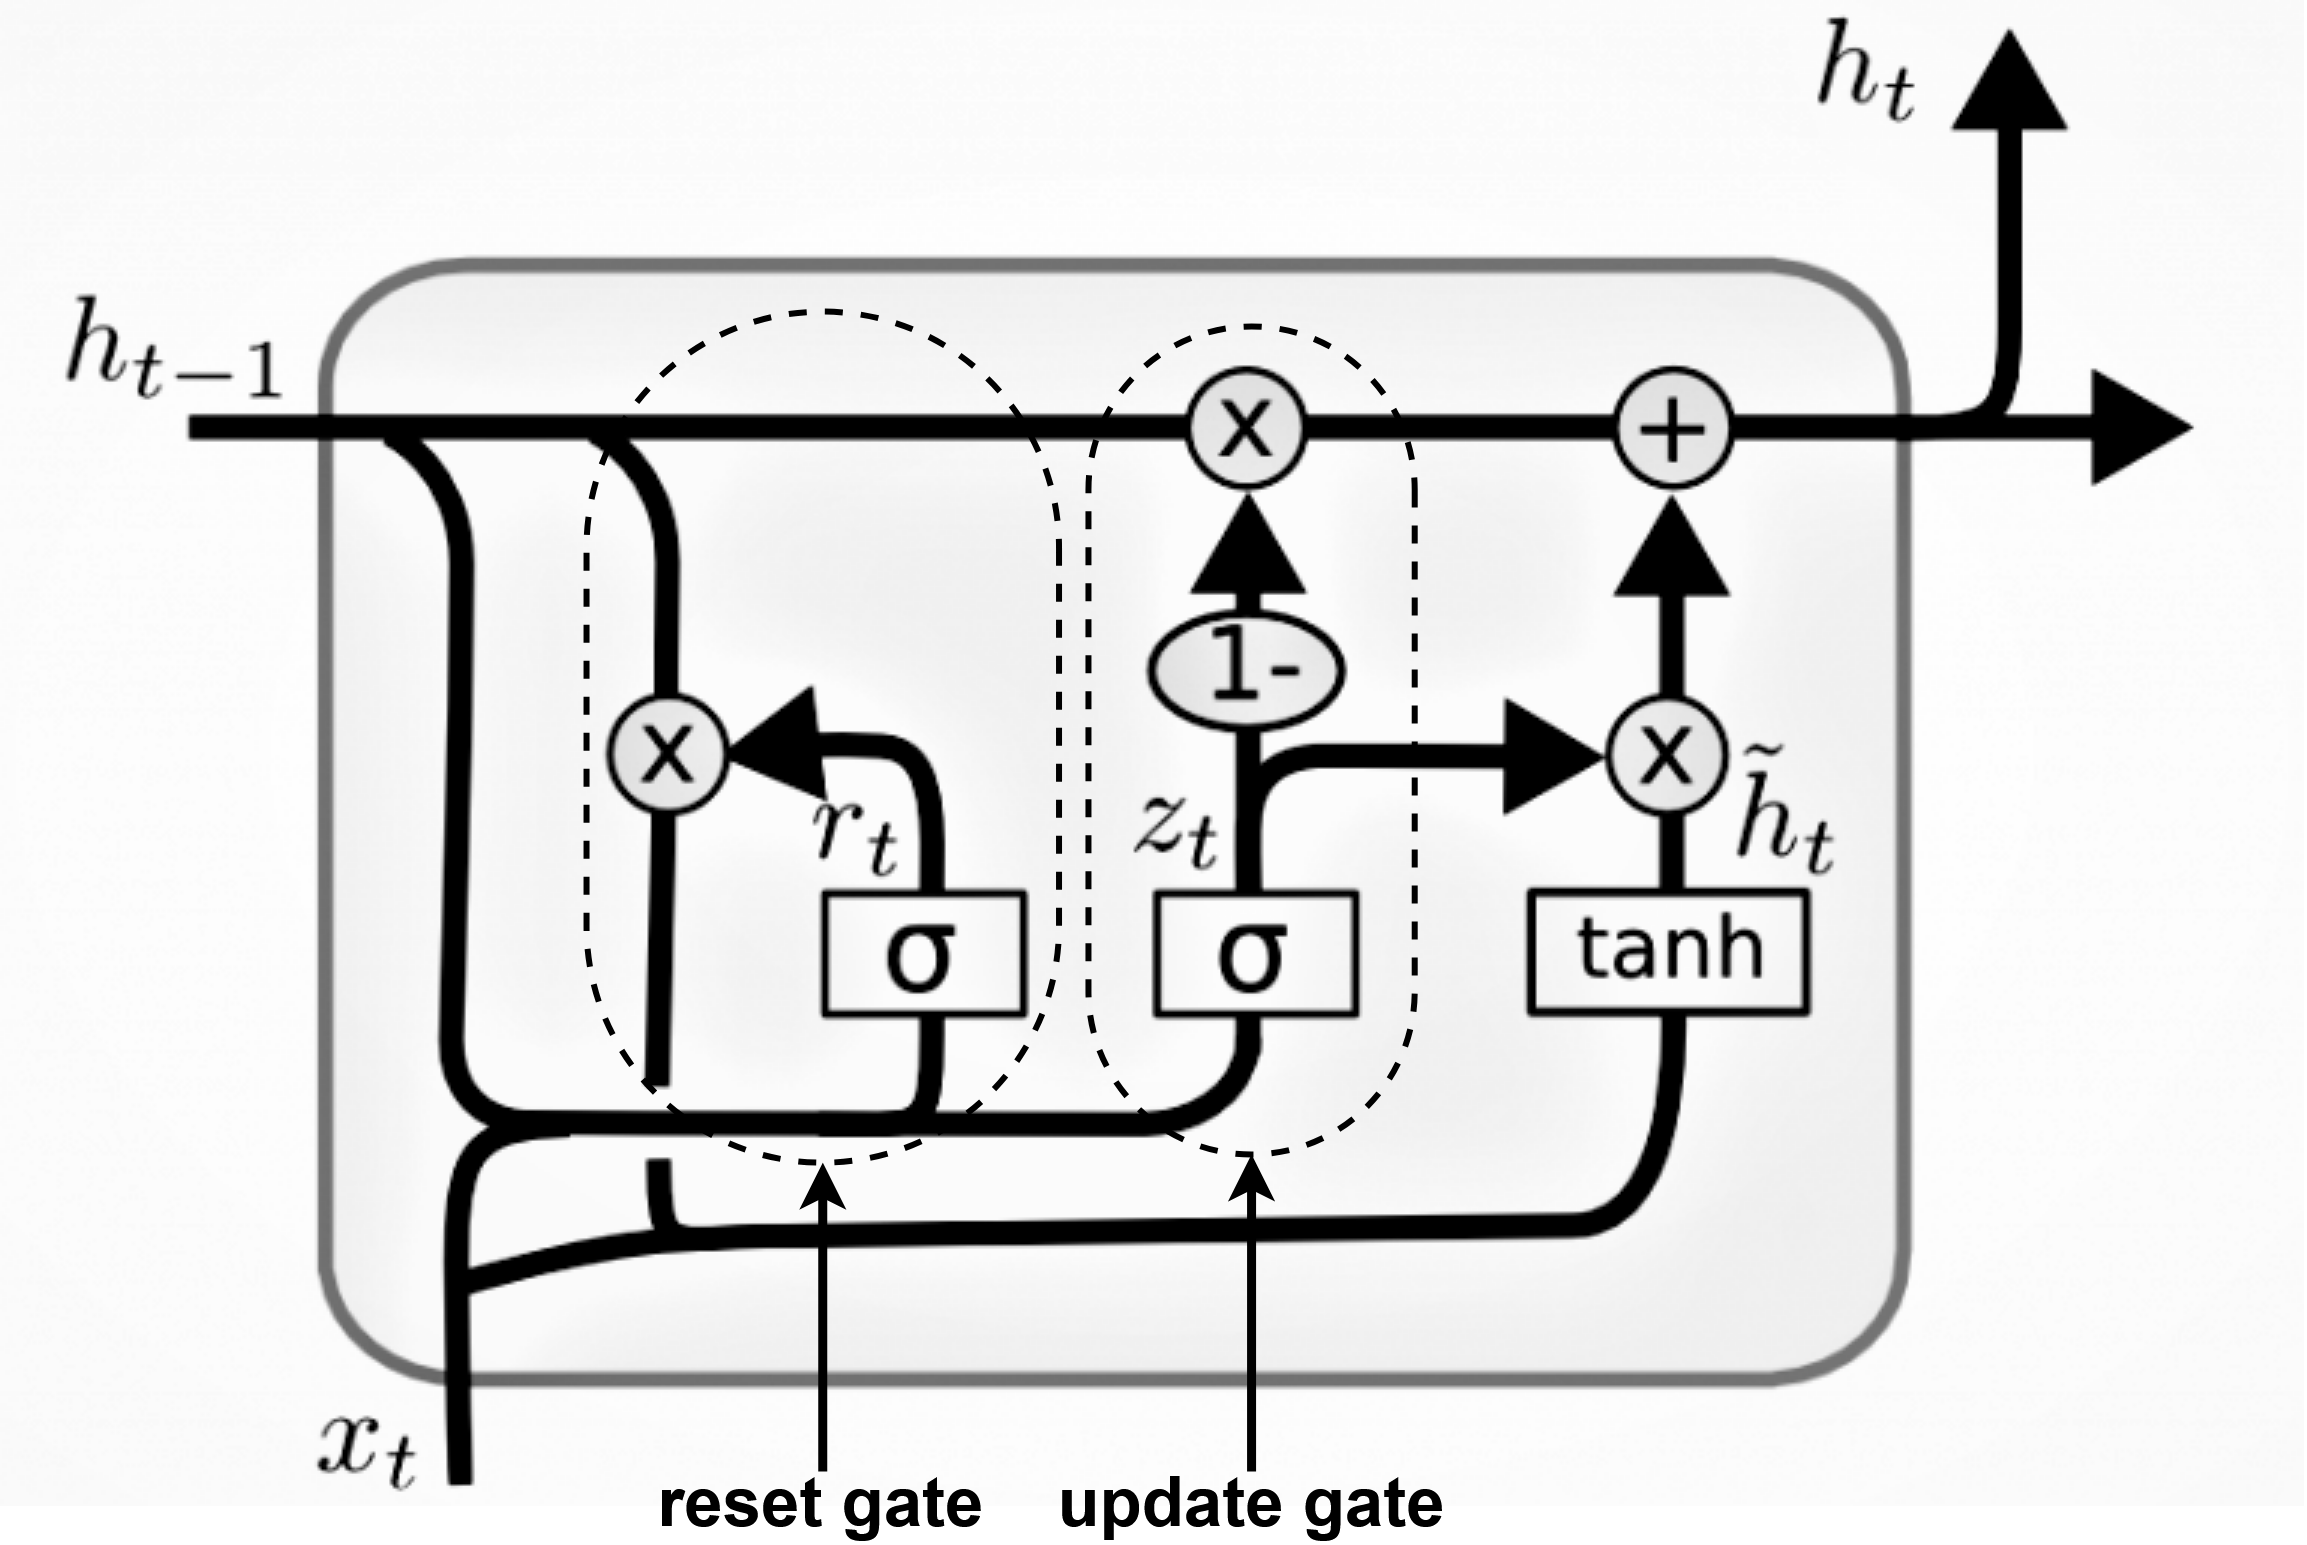
\includegraphics[width=0.6\textwidth]{Images/GRU_cell_detailed.png}
    \caption{GRU unit.}
    \label{gru}
    \end{center}
\end{figure}

The equations that describe the operation of a \ac{GRU} unit are given by 

\begin{equation}
    \begin{cases} 
        
        z_t = \sigma(W^{(z)} x_t + U^{(z)} h_{t-1} + b^{(z)})\\
        r_t = \sigma(W^{(r)} x_t + U^{(r)} h_{t-1} + b^{(r)})\\
        \tilde{h}_t = \tanh(W^{(h)} x_t + U^{(h)} h_{t-1} \circ r_t + b^{(h)})\\
        h_t = (1-z_t) \circ h_{t-1} + z_t \circ \tilde{h}_t

    \end{cases} ,
\end{equation}

where $zt$ represents the update gate vector, $r_t$ the reset gate vector, $\tilde{h}_t$ the candidate activation vector and $h_t$ the output vector. \ac{GRU}s have fewer tensor operations to perform, and so they take less time to train than \ac{LSTM}s.  

\subsubsection{One dimensional convolutional neural network (1D CNN)}\label{chap3:subsubsec:1dcnn}


Convolutional Neural Networks (\ac{CNN}s) are biologically-inspired feed-forward neural networks that have been successfully applied in the field of computer vision and digital image processing and analysis \cite{cnn0}.

In \ac{ML} applications, \ac{2D CNN} are typically used for categorizing 2D images (into classification problems) or creating images (in case of regression-based problems). In this kind of applications, the layers extract two-dimensional pathces from an image and then apply similar transformations to each of the patches. Similarly, there are \ac{1D CNN}, that extract data subsequences from a dimension of the main sequence. This thesis aims to predict the future behavior of certain variables of a single dimension, so that models consisting of \ac{1D CNN}'s layers have been tested.

The \ac{1D CNN} is very effective when you expect to derive interesting features from shorter (fixed-length) segments of the overall data set. Its main purpose is to turn the long input sequence into much shorter (downsampled) sequences of higher-level features, which can be very useful in the treatment of large time sequences.

In Figure \ref{conv1}, the reader may find a representation of the normal working process of a \ac{1D CNN}. The operation of \ac{1D CNN} is based on the extraction of odd size pathces (in this particular case it uses a convolution window with size 5), from a sequence of large dimensions of input data. Is then applied a convolution operation that can be written as \cite{cnn2} 

\begin{equation}
y(n)=
    \begin{cases} 
            
        \sum_{i=-\frac{k}{2}+\frac{1}{2}}^{\frac{k}{2}-\frac{1}{2}} x(n+i)h(i),\  if \  n=0.\\
        \sum_{i=-\frac{k}{2}+\frac{1}{2}}^{\frac{k}{2}-\frac{1}{2}} x(n+i+(s-1))h(i),\  otherwise.\\
    
    \end{cases} ,
\end{equation}

where $n$ represents the length of the convolution layer, $x$ represents the input of the layer, $h$ represents the kernel (or extracted patch) and $k$ its length. Lastly, $s$ represents the number of shifted positions of the kernel window after each convolution, also known as number of strides. For example, if n = 20, k=5 and s=1 then

\begin{equation}
    \begin{cases} 
        y(2)=x(0)h(0)+x(1)h(1)+x(2)h(2)+x(3)h(3)+x(4)h(4)\\
        y(3)=x(1)h(0)+x(2)h(1)+x(3)h(2)+x(4)h(3)+x(5)h(4)\\
        \  ...\\
        y(17)=x(15)h(0)+x(16)h(1)+x(17)h(2)+x(18)h(3)+x(19)h(4)\\
    \end{cases} .
    \label{noncausal}
\end{equation}

It should be mentioned that the output ($o=16$) does not have the same dimension as the input layer ($n=20$). This happens because no padding has been applied to the convolution which implies that for the length of the convolution layer $n$, the kernel size $k$, and the number of strides $s$, the output $o$ is given by:

\begin{equation}
    o = \lfloor \frac{(n-k)}{s} \rfloor + 1 .
\end{equation}

By applying "padding", having the input $n$, kernel size $k$, and padding with length $p$, the output $o$ is given by:

\begin{equation}
    o = \lfloor \frac{(n+2p-k)}{s} \rfloor + 1 .
\end{equation}

This allows to obtain \ac{1D CNN}'s layers whose input size is equal to the output. In this example, for the output $o$ dimension to have the same dimension as the input sequence, 20, then the $p$ dimension must be 2. In Figure \ref{conv1} it can be seen schematically the result of the described convolution operation.

\begin{figure}[h!]
    \centering
    \begin{center}
    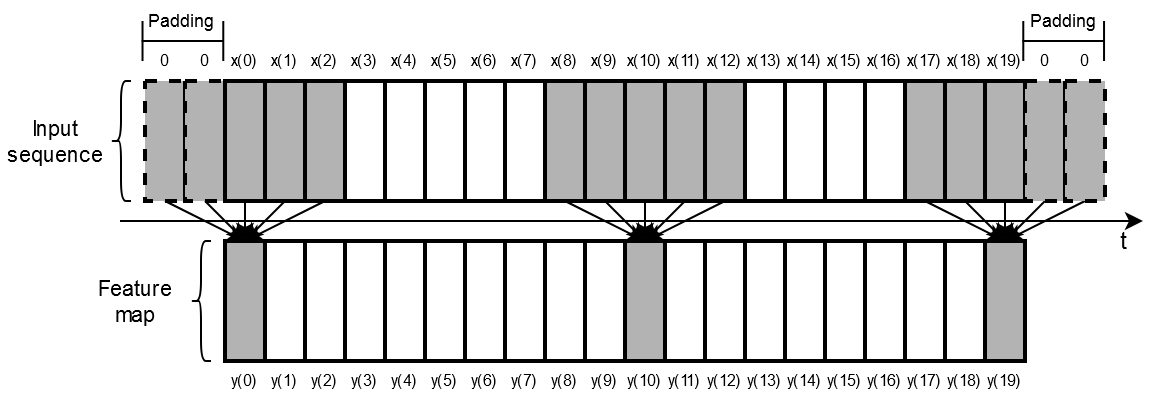
\includegraphics[width=1\textwidth]{Images/conv1.png}
    \caption{1D convolution working process.}
    \label{conv1}
    \end{center}
\end{figure}

Although it may seem like a good methodology, the convolution operation presents a particularity: it uses future values in its computing procedure. In the example present in Figure \ref{conv1}, it can be observed that in the computation of $y(10)$, for example, values of $x(8)$, $x(9)$, $x(10)$, $x(11)$ and $x(12)$ were used. In a series with time dependencies such as the problem in question, the use of future values in the computation of a present value presents an obvious violation, in which the output of instant $[t]$ depends on the input of $[t+1:]$. In this sense, the concept of causal convolution must be introduced. 

In causal convolution, the value of the generated output is not dependent on future inputs. In the same way described above, the causal convolution is given by 

\begin{equation}
y(n)=
    \begin{cases} 
            
        \sum_{i=0}^k x(n-i)h(i),\  if \  n=k-1.\\
        \sum_{i=0}^k x(n-i+(s-1))h(i),\  otherwise.\\
    
    \end{cases} ,
\end{equation}

where $n$ represents the length of the convolution layer, $x$ represents the input of the layer, $h$ represents the kernel (or extracted patch) and $k$ its length. Lastly, $s$ represents the number of shifted positions of the kernel window after each convolution, also known as number of strides. For example, if n = 20, k=5 and s=1 then

\begin{equation}
    \begin{cases} 
        y(4)=x(4)h(0)+x(3)h(1)+x(2)h(2)+x(1)h(3)+x(0)h(4)\\
        y(5)=x(5)h(0)+x(4)h(1)+x(3)h(2)+x(2)h(3)+x(1)h(4)\\
        y(6)=x(6)h(0)+x(5)h(1)+x(4)h(2)+x(3)h(3)+x(2)h(4)\\
        \  ...\\
        y(19)=x(19)h(0)+x(18)h(1)+x(17)h(2)+x(16)h(3)+x(15)h(4)\\
    \end{cases} .
    \label{noncausal}
\end{equation}

In Figure \ref{conv2}, a schematization of the causal convolution process can be seen.

\begin{figure}[h!]
    \centering
    \begin{center}
    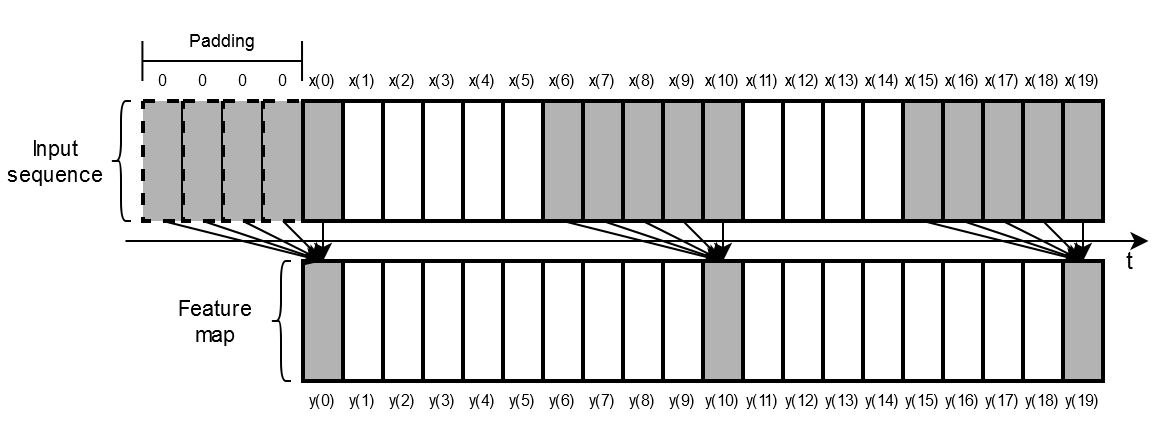
\includegraphics[width=1\textwidth]{Images/conv2.png}
    \caption{1D causal convolution working process.}
    \label{conv2}
    \end{center}
\end{figure}

In this layer category, convolutional windows are used, which is similar to using a k-dimensional kernel where all its elements have the value $\frac{1}{k}$. Following the example, with the kernel described in dimension 5, $y(19)$ is given by
\begin{equation}
        y(19)=x(19)\frac{1}{5}+x(18)\frac{1}{5}+x(17)\frac{1}{5}+x(16)\frac{1}{5}+x(15)\frac{1}{5}.
    \label{19}
\end{equation}



Usually, along with the \ac{CNN} layers, pooling layers are used. The pooling operation aims to simplify convolution output, giving more importance to prominent features. There are several types of pooling, the most important of which is Max pooling which involves selecting the largest value in a user-defined size window, thus reducing the dimensionality of the output. Following the example, for a $pool\_size$ of 5 units, one can see in Figure \ref{maxpooling}, the representation of the Max pooling operation where the dark units have the highest value within the 5-unit window. For the first 10 time-setps, the highest value value is then passed as layer output, and the dimension of the output decreases. In other words, for each set of 5 values, the largest is chosen, and the size of the output decreases with an inverse relationship to the chosen $pool\_size$. In this case, the dimensionality of the output decreases five times.

\begin{figure}[h!]
    \centering
    \begin{center}
    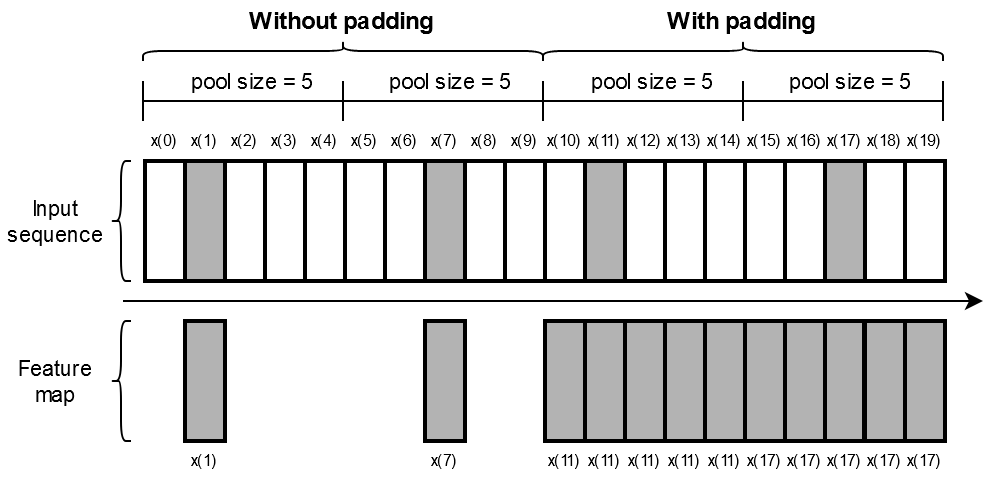
\includegraphics[width=0.9\textwidth]{Images/maxpooling.png}
    \caption{Max pooling without and with padding.}
    \label{maxpooling}
    \end{center}
\end{figure}

As for the problem under study in this thesis, it is essential to maintain the dimensionality of the input data. To accomplish this, padding was added to this layer. In Figure \ref{maxpooling}, for the last 10 time-steps, it is possible to observe Max pooling with padding, where the beginning of the process is similar as pooling without padding, but inside the output windows of dimension $pool\_size$, the higher selected value is copied to all the remaining empty spaces. 

In order to aggregate all the information covered in this section, the transformation that the data undergo, from the moment they serve as input to the 1D CNN, until the moment when the Max pooling  is performed, is portrayed in Figure \ref{resdata}.

\begin{figure}[h!]
\captionsetup[subfigure]{position=b}
\centering
\subcaptionbox{\label{inputseq}}{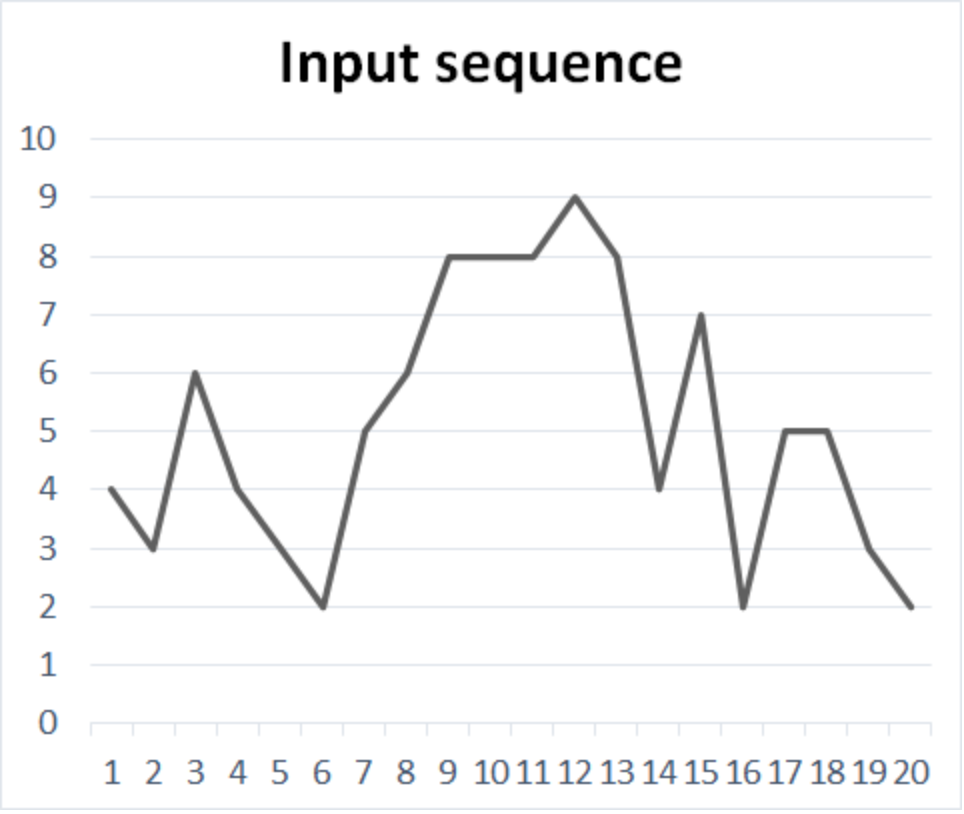
\includegraphics[width=.32\linewidth]{Images/inputsequence.png}}
\subcaptionbox{ \label{afterconv}}{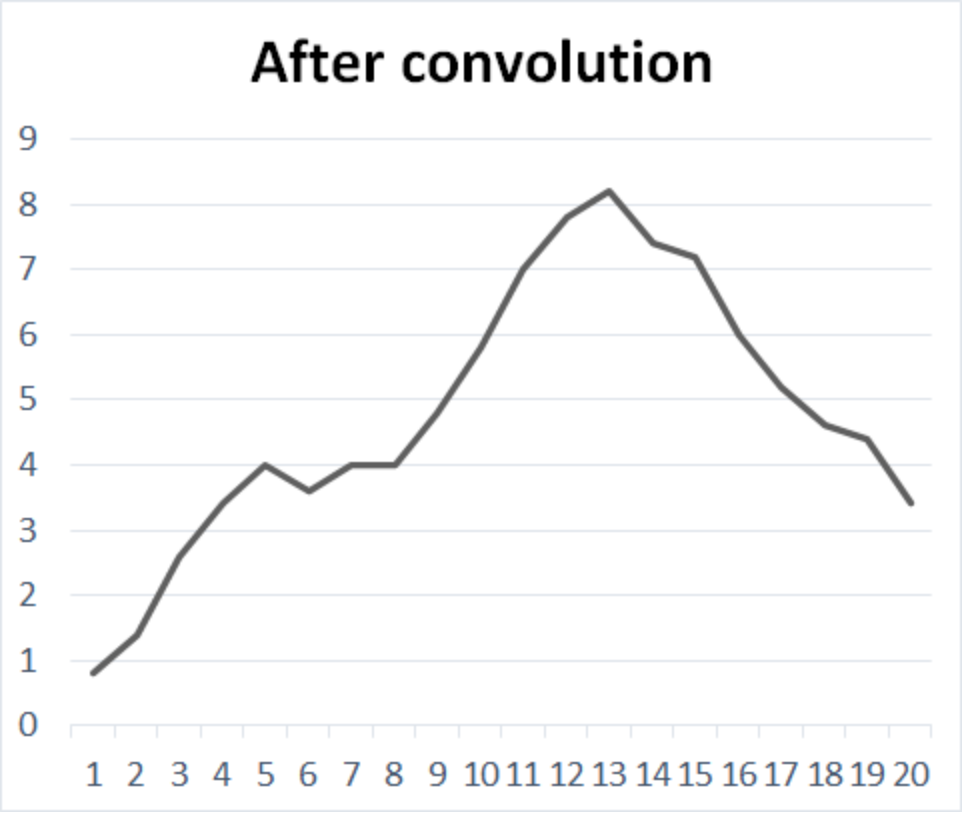
\includegraphics[width=.32\linewidth]{Images/afterconvolution.png}}
\subcaptionbox{ \label{aftermaxp}}{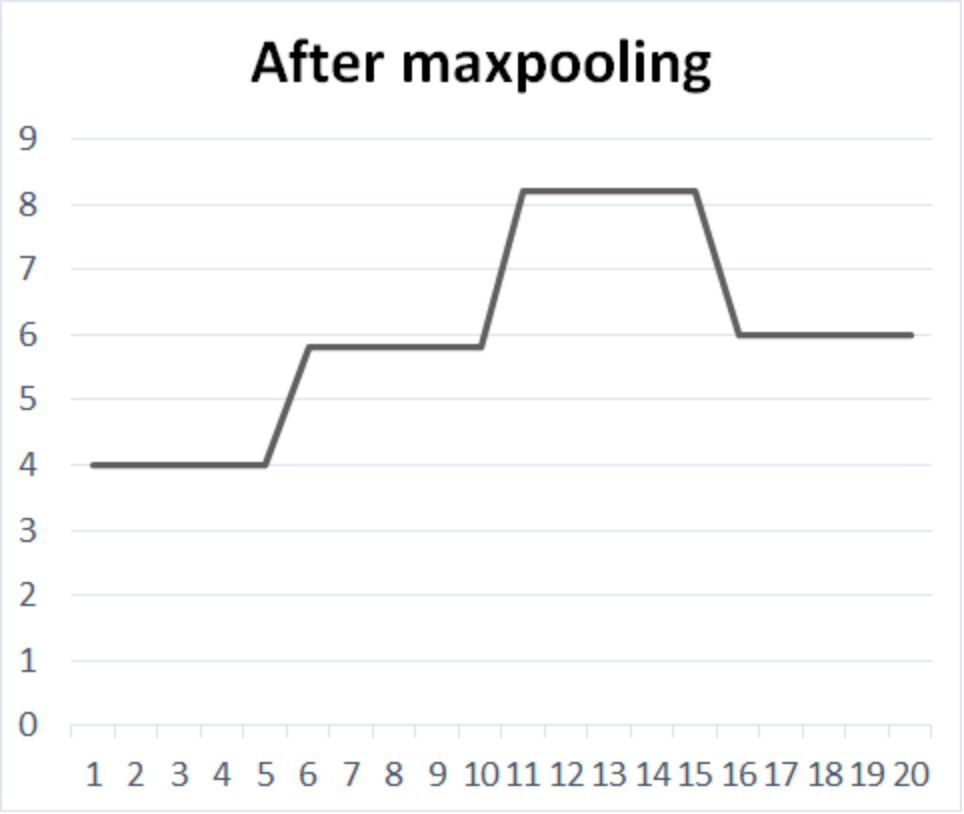
\includegraphics[width=.32\linewidth]{Images/aftermaxpooling.png}}
\caption{Example data a) Before convolution b) after convolution c) after Max pooling.}
\label{resdata}
\end{figure}


Figure \ref{inputseq} shows a 20 time-steps random signal, as the one used in the other examples used in this section. At this stage, the signal is in its original form, without any treatment. Figure \ref{afterconv} represents the result after the convolution operation with $kerne\_size$ 5. It can be seen that at this point, the signal is a smooth representation of the initial signal. The convolution operation extracts the main characteristics of the signal, ignoring intermediate oscillations. Afterwards, the Max pooling operation with $pool_size$ 5 is applied to the signal resulting from the convolution operation. The result of this operation is represented in Figure \ref{aftermaxp}, which consists of extending the point with the highest value within each of the 4 defined windows. This is the final signal resulting from the convolution operation with Max pooling, a simplified representation of the initial sequence.

\subsection{Networks specifications}\label{chap3:subsec:networks_specifications}

The process of designing the architectures to be tested is a complex and demanding task. This section describes the architectures used, as well as some techniques used in their development.

\subsubsection{Studied architectures}\label{chap3:subsubsec:studied_architectures}
In the development of this thesis, different types of neural networks were tested, composed of the layers introduced in section \ref{chap3:subsec:artificial_neural_networks}. The objective was to study the influence that each of the three layers introduced has on a predictive model, and to study the results obtained by pairing multiple layers into a single model. In Figure \ref{models}, are represented the five main architectures studied.

\begin{figure}[h!]
    \centering
    \begin{center}
    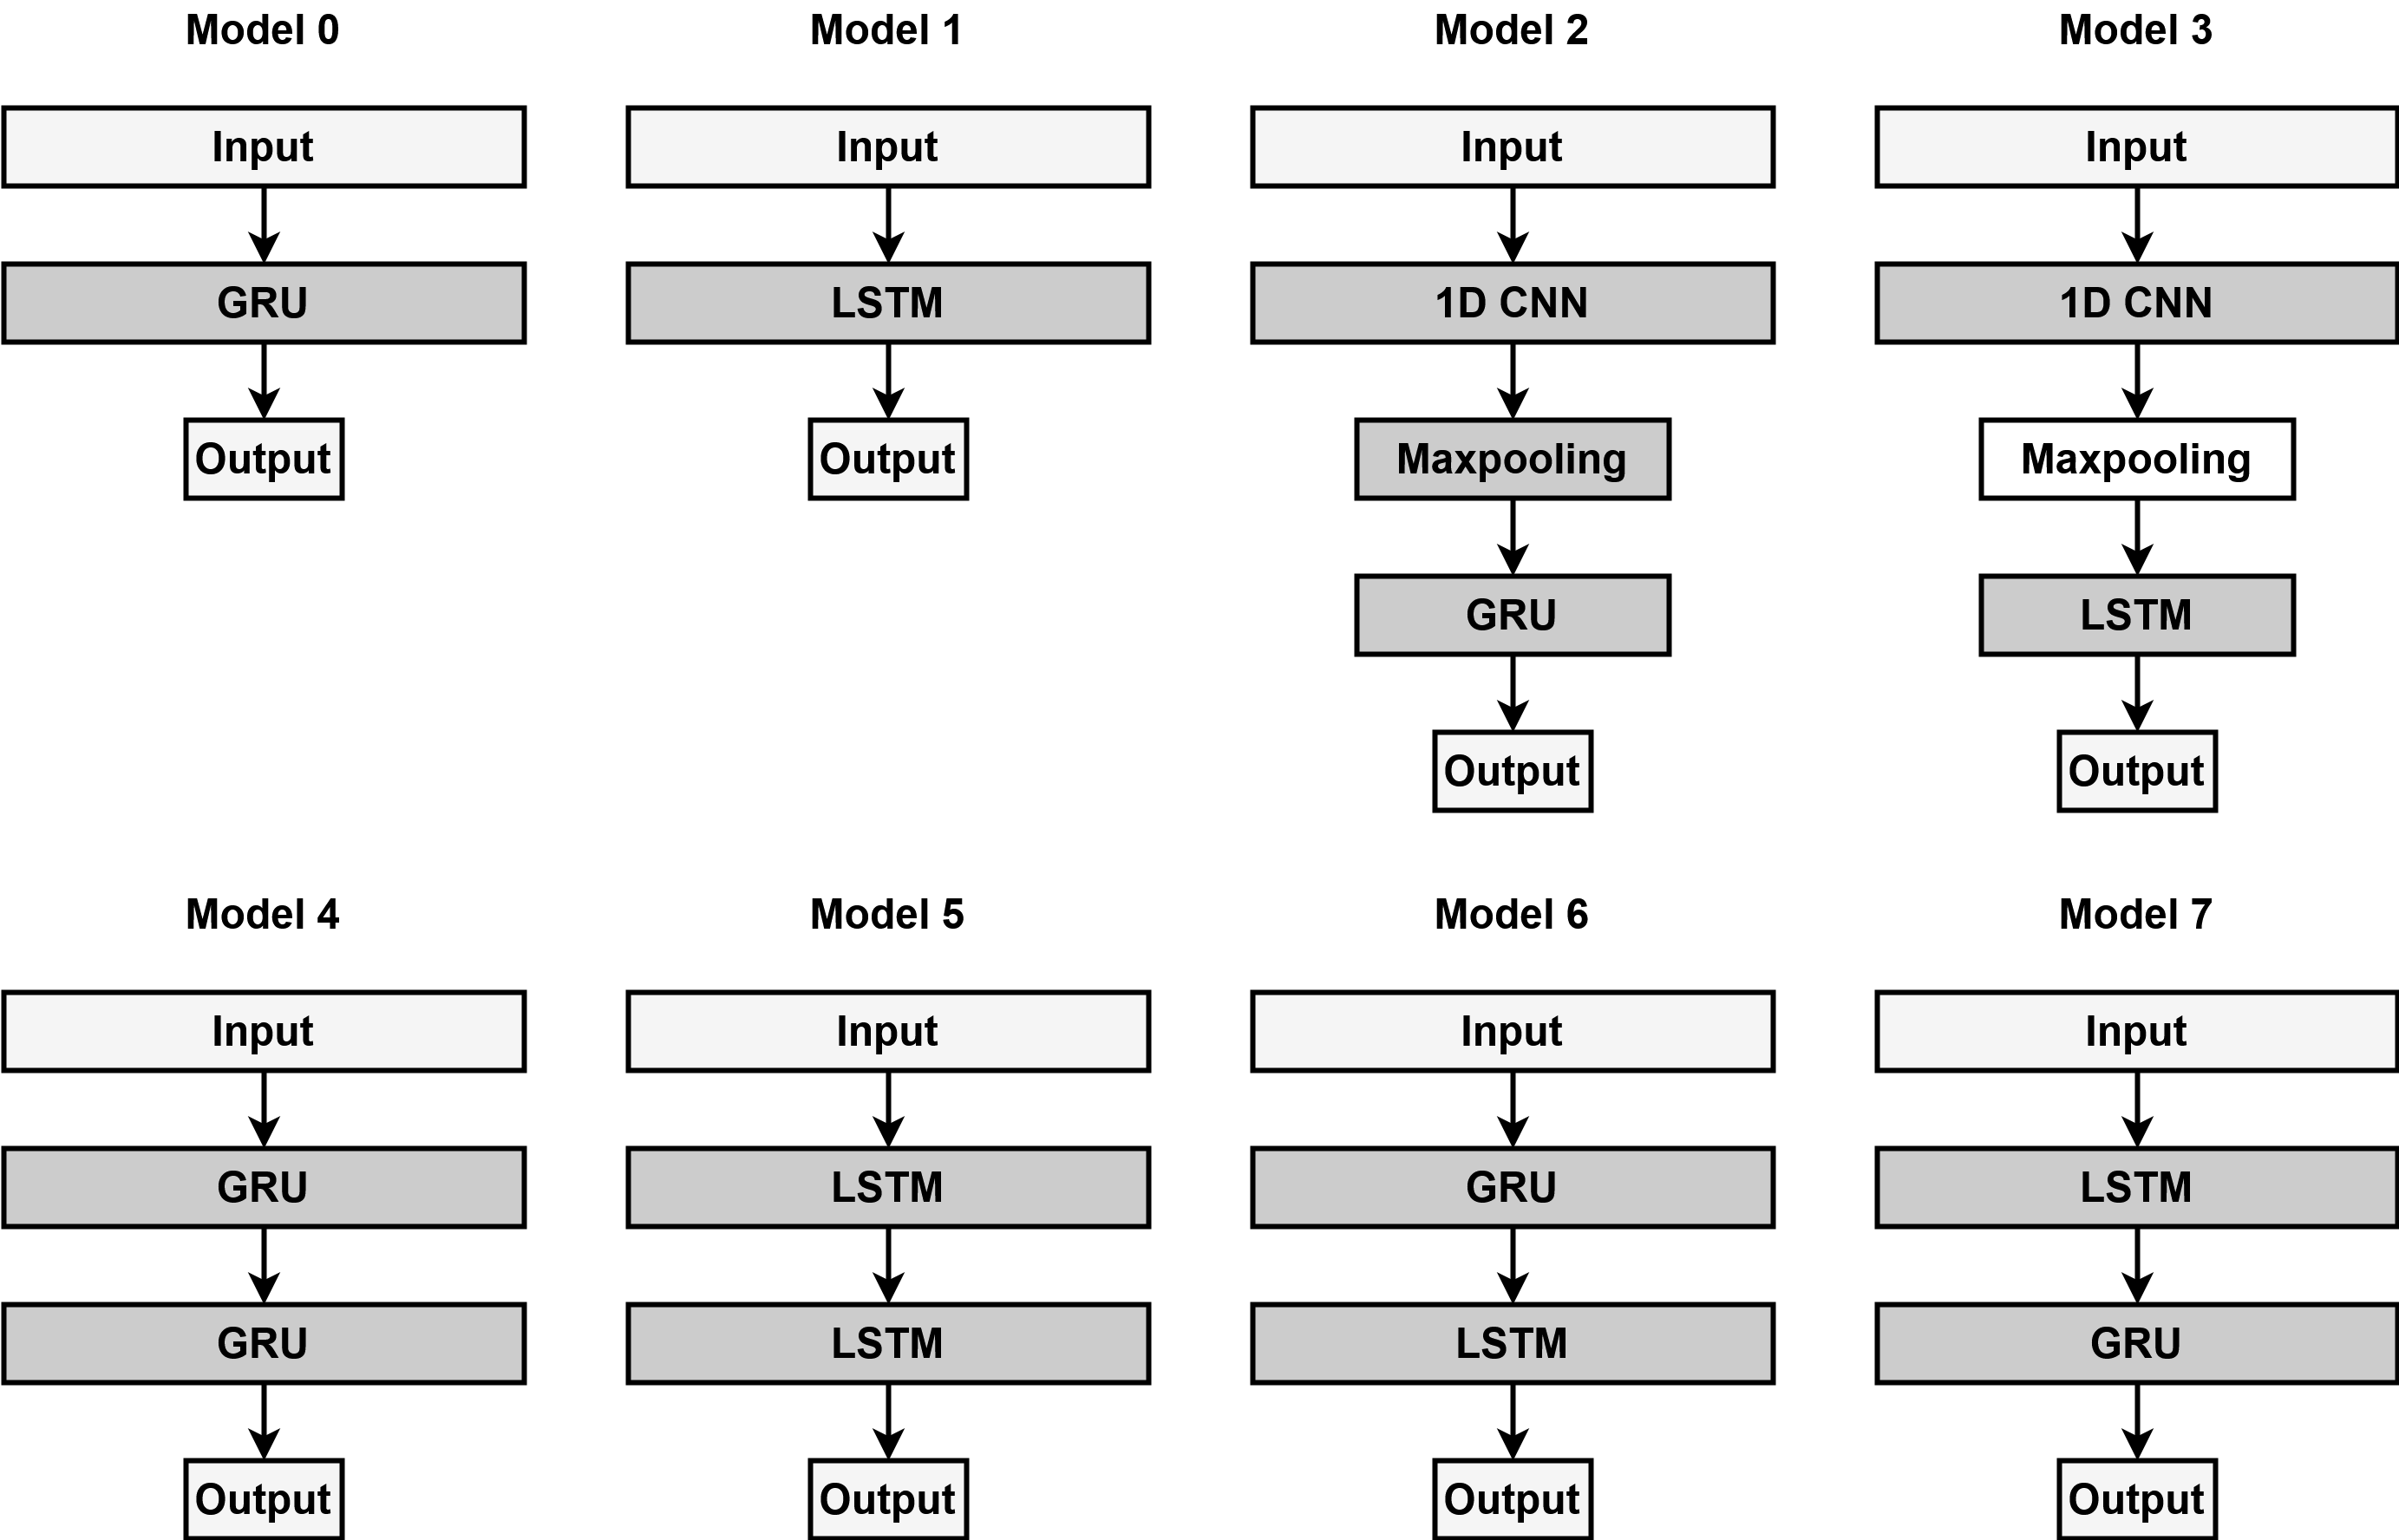
\includegraphics[width=1\textwidth]{Images/models.png}
    \caption{Tested model architectures.}
    \label{models}
    \end{center}
\end{figure}

Model 1, Model 2 and Model 3 are composed of a single layer of \ac{GRU}, \ac{LSTM} and \ac{1D CNN} respectively. The purpose of these three models is to compare the performance between the three types of single layer. In order to study the effect that the combination of \ac{CNN}s with \ac{GRU}s and\ac{LSTM}s has, the architecture of Model 4 is similar to that of Model 1, with the addition of a \ac{1D CNN} layer and a Maxpooling layer before the \ac{GRU} layer. Similarly, Model 5 is like to Model 2 with the addition of \ac{1D CNN} layer and a Maxpooling layer before the \ac{LSTM} layer. All five architectures present, as their last layer, a Dense layer with three units, responsible for converting the outputs of the previous layers into only three outputs, one for each of the forecasts ((t+5), (t+10) and (t+15)).


\subsubsection{Hyperparameter optimization} \label{chap3:subsubsec:hyperparameter_optimization}

A hyperparameter is a parameter whose value is used to control the learning process. Hyperparameter optimization is the process of choosing a set of optimal hyperparameters for a learning algorithm. Depending on the layer in question, different hyperparameters can be tuned. Other parameters, such as node weights are initialized randomly, and are defined during the learning process. In other words, hyperparameters are parameters which must be changed by the user according to the results obtained, while other parameters should not be modified by the user, and are the result of the learning process.

\ac{ANN}s have numerous advantages, both in terms of their usage and performance. On the other hand, tuning the hyperparameters is an extremely time-consuming process that is done by hand. A certain set of hyperparameters is trained, validated, and then changed and so on until the best possible result is obtained. During the tests performed with the models present in Figure \ref{models}, different hyperparameters were tuned such as the number of nodes in each layer, number of filters of each \ac{1D CNN} layer and kernel size.

\subsubsection{Regularization techniques}\label{chap3:subsubsec:regularization_techniques}

During the learning process of an \ac{ANN}, it is possible that overfitting occurs. Overfitting is a term used to describe when a model fits very well to the previously observed data set, but proves to be ineffective in predicting new results. In practice, overfitting causes the model to perform very well during training, but the performance gets much worse when faced with brand new data because the model has adapted too much to the training data.  

Regularization refers to a set of different techniques that lower the complexity of a neural network model during training, and thus prevent the overfitting \cite{reg0}. There are several types of regularization techniques. In this thesis, two techniques were used: Early-stopping and Dropout.

\paragraph{Early-stopping}\label{sec:early}

Early-stopping is probably the most common regularization technique. In Figure \ref{early} the reader can find a two graphs that portray the evolution of the error over epochs of a prediction model. During the training and validation process of the predictive models, the error associated with the training set tends to decrease with the increase of the number of training epochs. In an optimal case, with the increase of the number of validation epochs, the error associated with the training set also tends to decrease, thus reaching a trained and validated model whose error produced at validation is minimal. In the case of datasets large enough to overfit, it is observed that most of the time the training set error also tends to decrease, but the validation error starts to increase at a certain point. This is one of the main ways to identify overfitting.

\begin{figure}[h!]
\captionsetup[subfigure]{position=b}
\centering
\subcaptionbox{\label{early0}}{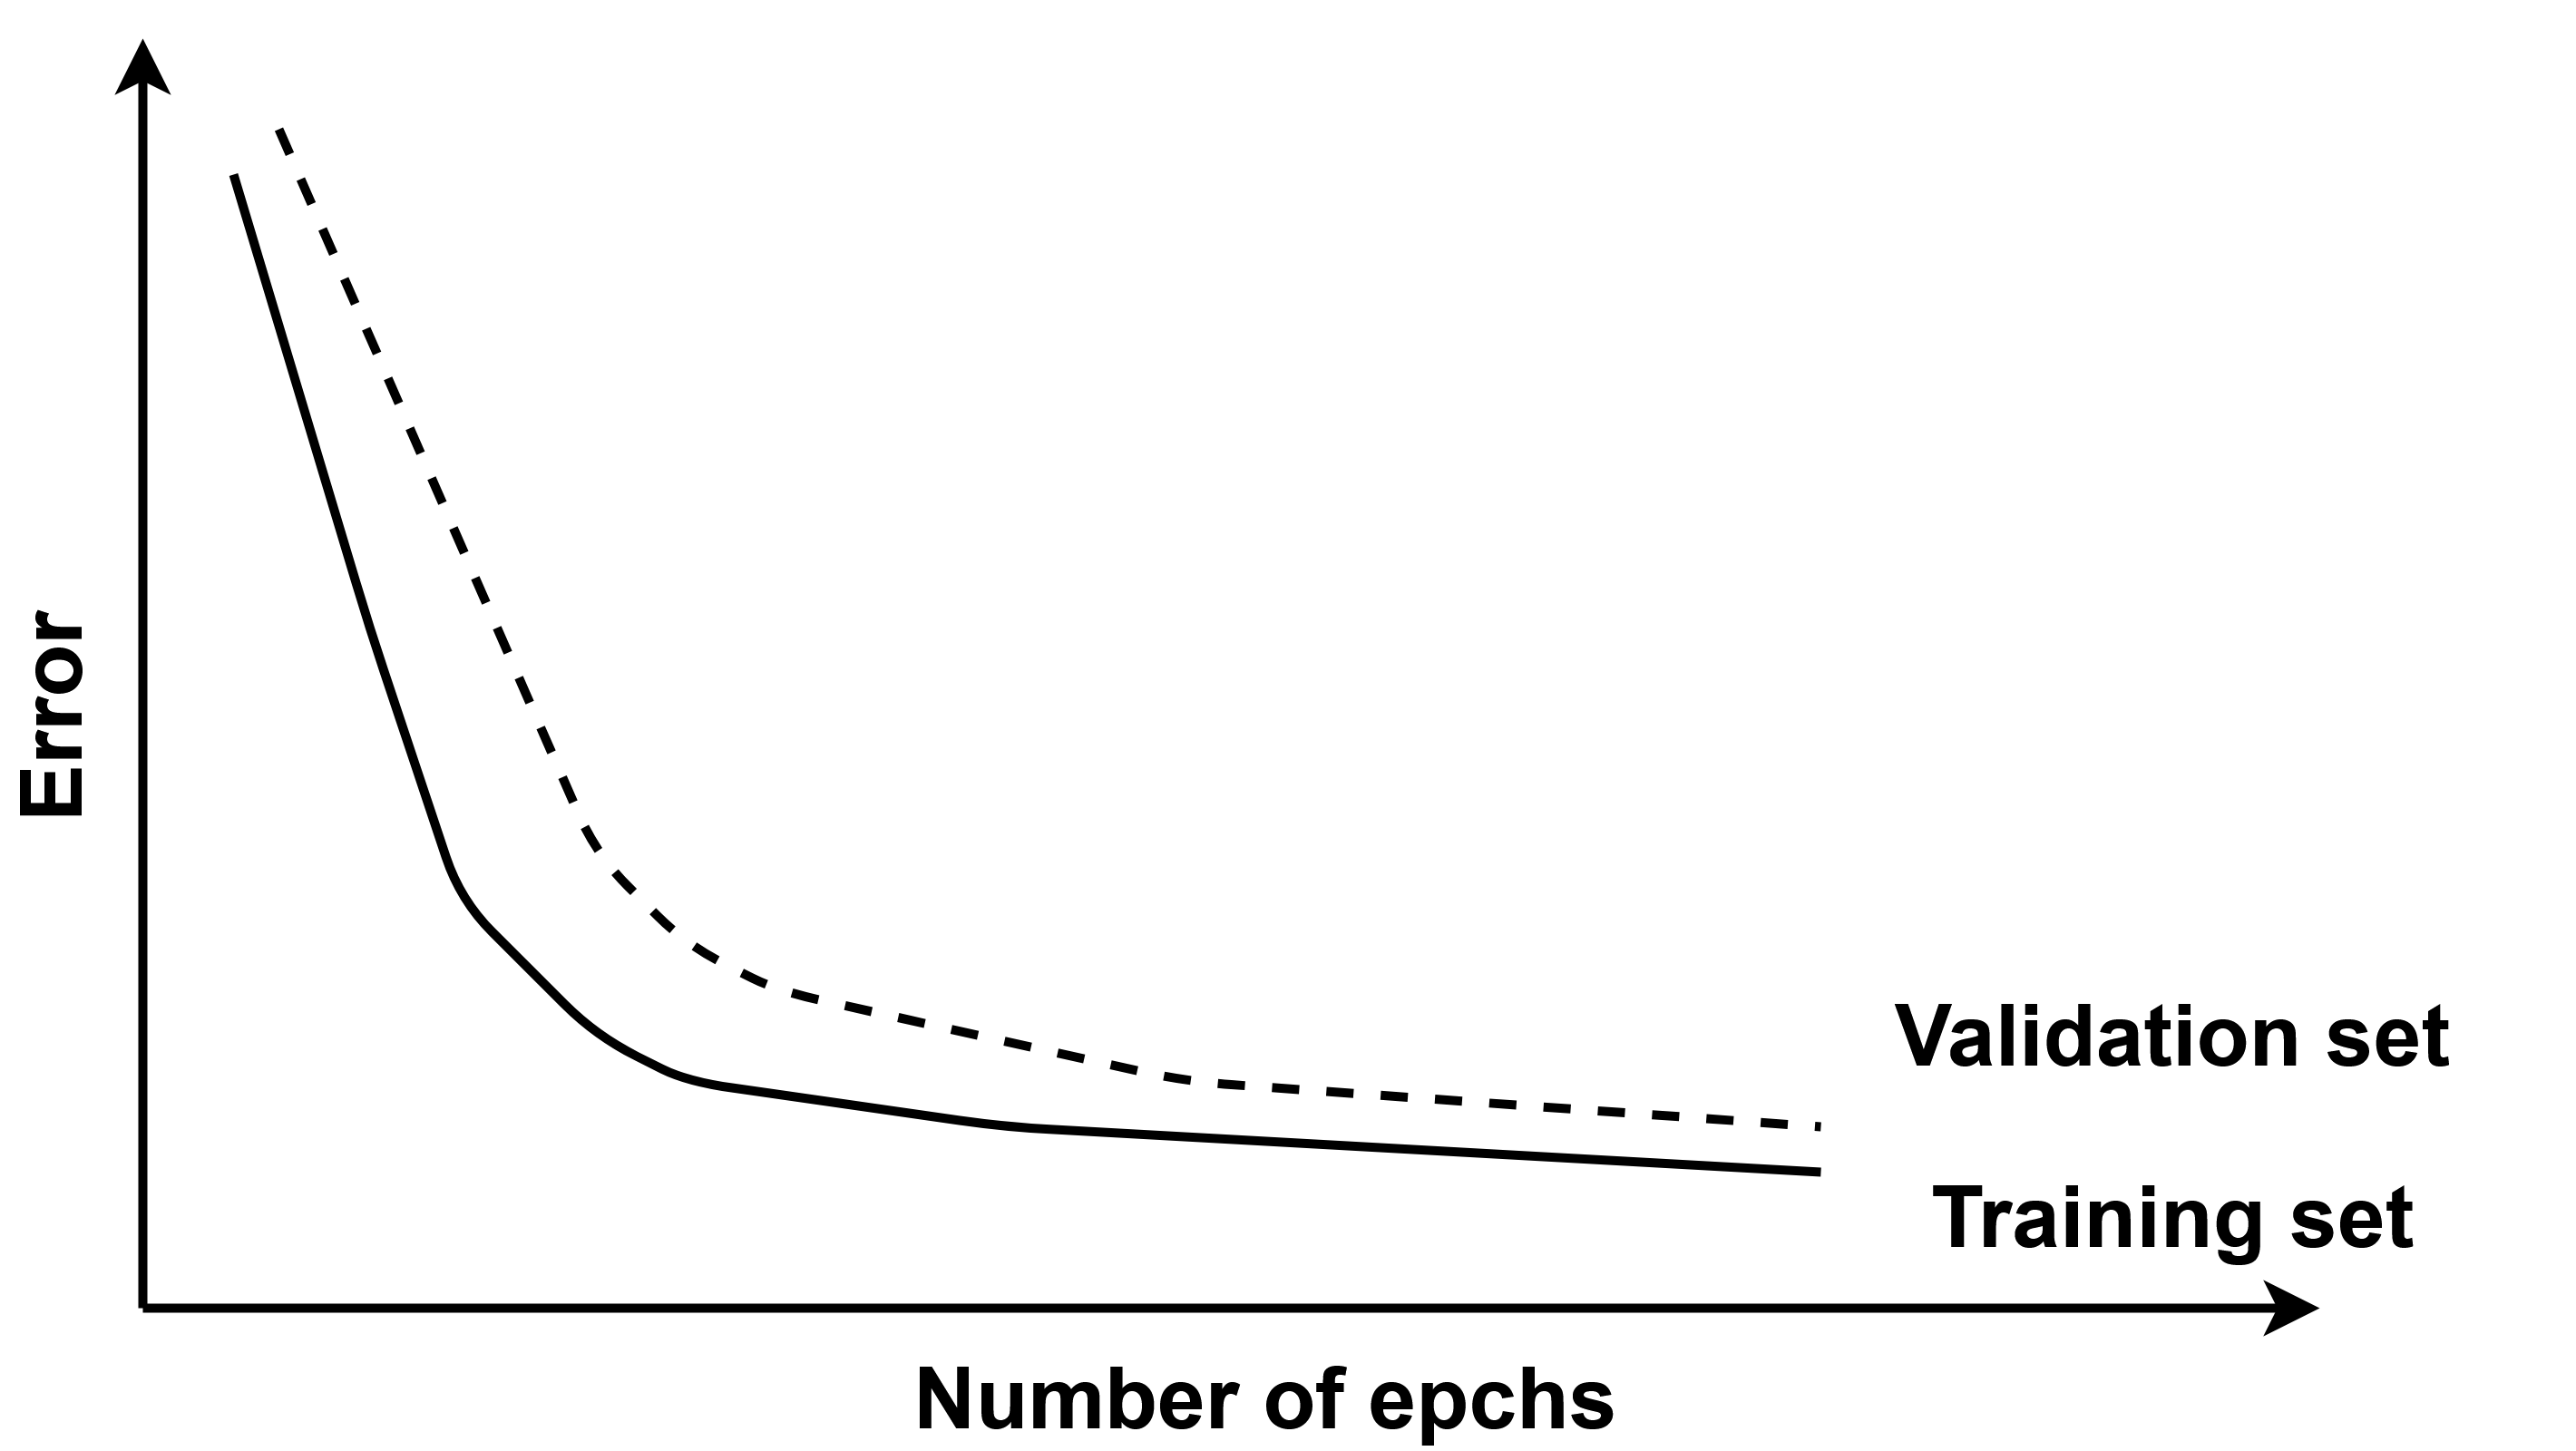
\includegraphics[width=.45\linewidth]{Images/early-stopping0.png}}
\hspace{0.05\textwidth}
\subcaptionbox{ \label{early1}}{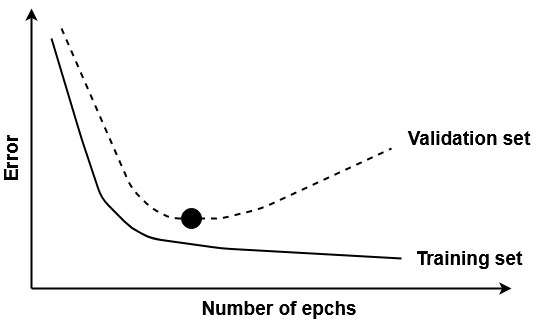
\includegraphics[width=.45\linewidth]{Images/early-stopping1.png}}
\caption{Prediction error evolution over epochs a) without overfitting b) without overfitting.}
\label{early}
\end{figure}

In Figure \ref{early0}, an ideal case is represented where there is no overfitting. It can be verified that the evolution of the validation error follows the evolution of the training error. Figure \ref{early1} presents a clear case of overfitting in which, at the moment marked with the black dot, the model presents its smallest validation error, which later increases. The early-stopping process consists in, from the moment the system detects that the validation error increases, it runs for more $p$ (patience factor) epochs where it gives the system the opportunity to obtain lower values of validation error. If in none of the $p$ epochs a lower value is found, the training process ends, eraly-stopping occurs. In the extreme case where $p$ = 0, the system stops the training process as soon as it detects a higher value than the previous one for the validation error, moment marked by the black circle present in Figure \ref{early1}.

\paragraph{Dropout}

In the process of training a fully connected \ac{ANN}, neurons tend to develop an interdependence between each other, which limits their individual capacity leading to overfitting.


To tackle this problem, the dropout is used, which is also widely used regularization technique. In Figure \ref{drop0} it is possible to see a \ac{ANN} without a dropout, and in Figure \ref{drop1} it is possible to see the same \ac{ANN} after dropout is applied.

\begin{figure}[h!]
\captionsetup[subfigure]{position=b}
\centering
\label{fig:drop}
\subcaptionbox{\label{drop0}}{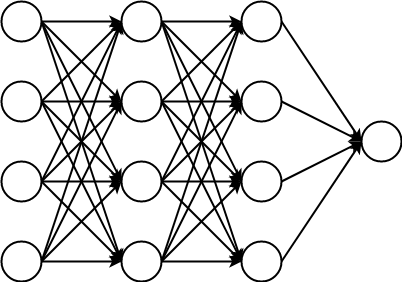
\includegraphics[width=.4\linewidth]{Images/dropout0.png}}
\hspace{0.05\textwidth}
\subcaptionbox{ \label{drop1}}{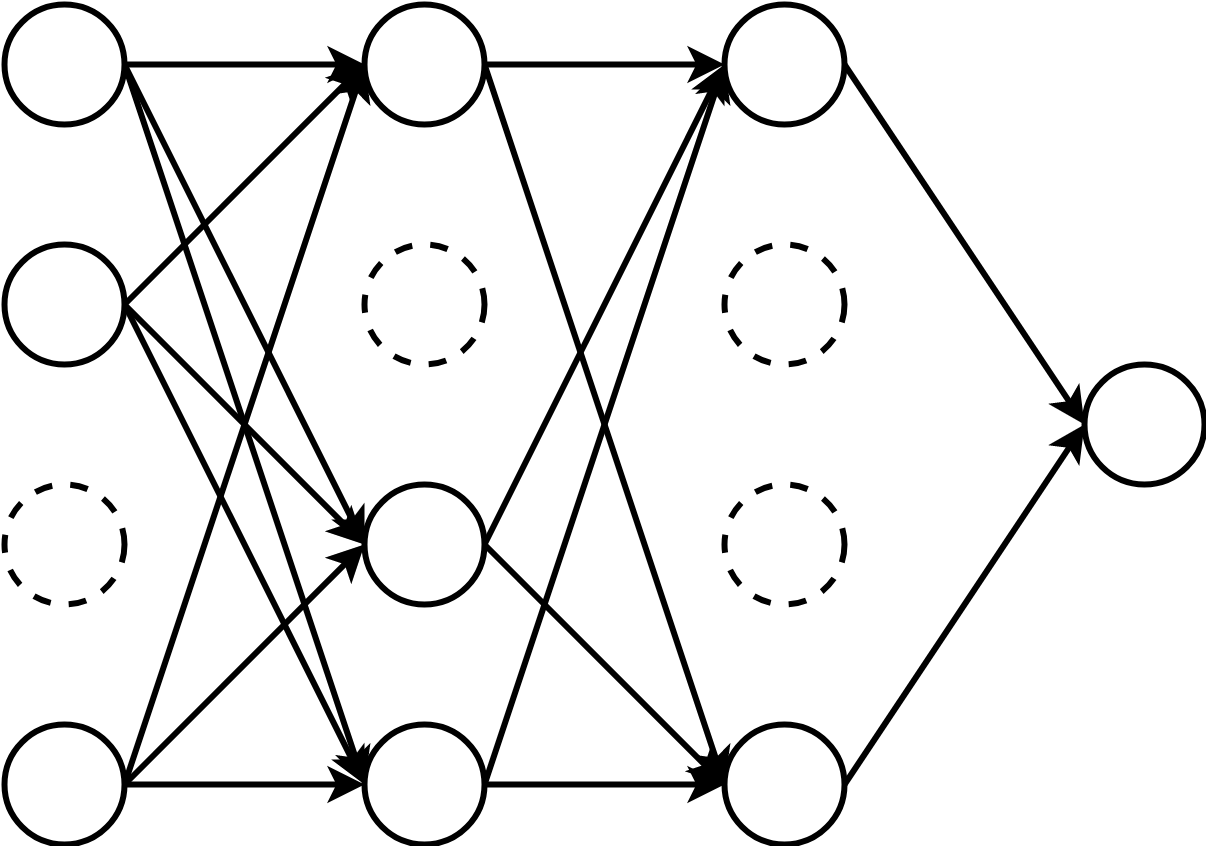
\includegraphics[width=.4\linewidth]{Images/dropout1.png}}
\caption{Artificial neural network a) without dropout b) with dropout.}
\end{figure}

The application of dropouts, implies for each hidden layer, for each sample of training, and for each iteration, to ignore a fraction $p$ of random neurons (and corresponding activations) during the training process. During the validation phase, all activations are then used, but reduced by a $p$ factor to take into account the missing activations lost during the training \cite{drop0}.

\section{Implementation environment}\label{chap3:sec:implementation_enviromnet}

During the development of the thesis, several scripts were implemented, both for data processing and for the implementation of machine learning models. The language chosen for this purpose was \textit{Pyhton}. The primary reasons for this choice were the ease of syntax of this language, as well as the large number of libraries available, including \textit{keras}, a Deep Learning library that provides all the necessary tools for building and deploying Neural Networks.

Regarding the hardware components used, two different systems were used during the development of this work. The first environment consists of a CPU (Intel Core i5-3470 3.20GHz), and a GPU (NVIDIA GeForce GTX 1050 Ti) essential to accelerate the training process of the proposed models. The second environment consists of a virtual environment implemented on \textit{Microsoft Azure Machine Learning} platform, where a cluster consisting of a 6 core processor, and a GPU (NVIDIA Tesla K80).

The first setup was used with the purpose of testing, in a first phase, several models with simple tasks, and the second environment was used to put into practice more complex tests that required more computational capacity.
	
\section{Performance evaluation metrics}\label{chap3:sec:performance_evaluation_metrics}

In the previous section, important details concerning the data used in this thesis were explained. One defined $Model\ error$, but did not specify which concrete metrics were used in this work. To compare the performance of the different models in the defined dataset, it is necessary to use some measures of forecast performance. In this sense, during this thesis four different measures were used that relate the real values present in the time series represented by $y_t$, and the forecast values, which are represented by $f_t$. Thus, the forecast error is given by $e_t=y_t-f_t$. The three measures presented are quite common in the literature \cite{} and are described below.

\subsection{Mean Absolute Error (MAE)}

The \ac{MAE}, is defined as

\begin{equation}
     MAE =\frac {\sum_{t=1}^n|e_t|}{n}.
\label{mae}
\end{equation}

The \ac{MAE} is known as a scale-dependent accuracy measure and measures the average absolute deviation between the forecasted values and the real ones. As a scale-dependent measure, it cannot be used to compare series series using different scales.


\subsection{Mean Squared Error (MSE) and Root Mean Squared Error (RMSE)}

The \ac{MSE}, is defined as

\begin{equation}
     MSE =\frac {1}{n}\sum_{t=1}^ne_t^2.
\label{mse}
\end{equation}

The \ac{MSE} is also known as a scale-dependent accuracy measure and measures the average squared deviation between the forecasted values and the real ones. The application of this measure is quite relevant because it doesn't allow the negative errors to cancel the positive errors and vice-versa. 

By applying the square root to the \ac{MSE}, the \ac{RMSE} is then defined as

\begin{equation}
     RMSE =\sqrt{MSE} = \sqrt{\frac {1}{n}\sum_{t=1}^ne_t^2}.
\label{rmse}
\end{equation}
Mathematically, the \ac{RMSE} is the square root of the average of the squared difference between the predicted values and the observed ones. The advantage of \ac{RMSE} over \ac{MSE} is that it is on the same scale as the targets, facilitating its interpretation in the concrete context of the problem. 

\ac{RMSE} and \ac{MAE} were the metrics implemented in the development of this research. These two measurements present some similarities, but also some differences that make it relevant to use the two metrics separately. In terms of similarities, both are expressed in the units of the variable in question, which means that both errors are easily interpretable given the context of the problem. The major difference between the two metrics lies in the contribution that individual error values make to the final result. In the case of \ac{MAE}, the contribution of individual errors follows a linear behavior. An error of 20 units contributes twice as much as an error of 10 units, and an error of 500 units contributes half as much as an error of 1000 units. In the case of \ac{RMSE} the errors are squared before being averaged, which means that this metric gives more weight to larger errors.  This means that very small errors tend to be ignored while large errors tend to be magnified. One can then conclude that \ac{RMSE} is especially useful when one intends to emphasize large errors and reduce the importance of smaller errors. It was then chosen to use both \ac{RMSE} and \ac{MAE} in the evaluation of the implemented models since both express interesting results that could be advantageous in the development of the research.

\section{Conclusion}\label{chap3:sec:conclusion}
